% -*- latex -*-
\documentclass[a4paper,12pt]{article}
\usepackage[utf8]{inputenc}
\usepackage[T1]{fontenc}
\usepackage[german]{babel}
\usepackage{lmodern}
\usepackage{amsmath,amssymb,amsthm}
\usepackage{geometry}
\usepackage{graphicx}
\usepackage[hidelinks]{hyperref}
\usepackage{booktabs}
\usepackage{listings}
\usepackage{xcolor}
\usepackage{enumitem}
\usepackage{microtype}
\emergencystretch=4em
\geometry{margin=2.5cm}
\setlength{\tabcolsep}{3pt}

\definecolor{mainblue}{RGB}{25, 70, 140}
\definecolor{accentred}{RGB}{180, 50, 30}
\definecolor{lightgray}{RGB}{245, 245, 248}
\definecolor{darkgray}{RGB}{60, 60, 70}
\definecolor{darkgreen}{RGB}{30, 100, 50}
 
\hypersetup{colorlinks=true, linkcolor=mainblue, citecolor=accentred, urlcolor=mainblue}

\title{\textbf{Wann ist das Datennetz gut genug für KI?}\\\large Eine ökonomische und formale Betrachtung des AI Data Network}
\author{\textsc{Stephan Epp}\\ {\small \texttt{\textbf{M.Sc.}}}}
\date{15. Oktober 2026}

% Theorem environments
\theoremstyle{definition}
\newtheorem{definition}{Definition}[section]
\newtheorem{bemerkung}[definition]{Bemerkung}
\newtheorem{satz}[definition]{Satz}
\newtheorem{lemma}[definition]{Lemma}
\newtheorem{korollar}[definition]{Korollar}

% Notation
\newcommand{\bits}{\{0,1\}}
\newcommand{\NN}{\mathbb{N}}
\newcommand{\RR}{\mathbb{R}}
\newcommand{\cP}{\mathrm{P}}
\newcommand{\cNP}{\mathrm{NP}}
\newcommand{\E}{\mathbb{E}}
\newcommand{\Var}{\mathrm{Var}}
\newcommand{\KL}{\mathrm{KL}}

\begin{document}
\maketitle

\begin{abstract}
Diese Arbeit untersucht, wann das Datennetz eines Unternehmens für eine konkrete KI-Anwendung gut genug ist. Ausgangspunkt ist nicht die Forderung nach fehlerfreien Daten, sondern eine ökonomische Abwägung: Ist der verbleibende Fehler im Verhältnis zu den Folgen der unterstützten Entscheidung vertretbar? Eine Fallstudie zur sinkenden Deckungsbeitragsmarge zeigt, wie eine plausibel klingende, aber unvollständige KI-Erklärung zu einer falschen Maßnahme führen kann, wenn Logistikdaten und Produktmix im Datennetz fehlen. Darauf aufbauend verbindet die Arbeit ein formales Modell von Datennetz, Data Product, Provenance und Error Budget mit einem praktischen Vorgehen. Sie beschreibt KI als Hinweis- und Prüfwerkzeug, vier stufenweise Vertrauensniveaus, ein Data Product als wiederverwendbare Grundlage, drei benannte Verantwortlichkeiten und messbare Kriterien für Fortschritt. Die zentrale These lautet: Abweichungen zwischen KI-Antwort und Unternehmensanalyse sind nicht nur ein Risiko, sondern können Datenlücken und zugleich mögliche Lücken in der eigenen Analyse sichtbar machen. Das Modell liegt als ausführbare, exakt rechnende Implementierung vor und wird experimentell geprüft: Die Fallstudie wird reproduziert (erklärter Anteil $3/22\approx 13{,}6\,\%$), die ökonomisch optimale Auswahl von Datenintegrationen erweist sich als Treppenfunktion des Budgets, bei der Abhängigkeiten zwischen Quellen die Rangfolge umkehren können, und der verwendete SAT-basierte Entscheider stimmt in allen 33 geprüften Fällen mit einer vollständigen Aufzählung überein, wächst aber exponentiell in der Zahl der Optionen. Die Zahlen beruhen auf einer illustrativen Fallstudie und auf Annahmen zu Kosten und Nutzen; sie sind Rechenbeispiele und kein empirischer Wirksamkeitsnachweis.
\end{abstract}

\tableofcontents
\newpage

\section{Einleitung}
Die drei leitenden Gedanken dieser Arbeit sind eng miteinander verbunden. Erstens hängt Vertrauen in eine Antwort nicht davon ab, ob sie vollkommen fehlerfrei ist, sondern davon, ob ein möglicher Fehler für den konkreten Verwendungszweck klein genug ist. Zweitens bezeichnet das Datennetz mehr als die Summe gespeicherter Daten: Entscheidend sind auch Verknüpfungen, Zugriffswege, gemeinsame Definitionen und Aktualität. Dasselbe KI-Modell kann deshalb auf einem gut verbundenen Netz nützliche und auf einem fragmentierten Netz irreführende Antworten geben. Drittens können KI-Antworten bereits vor vollständiger Datenreife als Hinweise und Gegenprüfung der eigenen wirtschaftlichen Analyse nützlich sein.

Diese Perspektive vermeidet zwei Extreme: KI-Antworten weder blind als Wahrheit zu übernehmen noch den Einsatz bis zu einer unerreichbaren Perfektion der Daten aufzuschieben. Stattdessen werden Nutzung und Autonomie nach den möglichen Folgen eines Fehlers gestuft. Die Arbeit führt zunächst in die Lücke zwischen KI-Ambition und Datenreife ein und erläutert eine Fallstudie zur sinkenden Marge. Danach folgen ein formales Modell, eine ökonomische Bedingung für ausreichende Qualität und ein Lernkreislauf für Abweichungen. Abschließend werden Data Products, Verantwortlichkeiten, Umsetzungsschritte, Unternehmensgrößen, Messgrößen und eine Go-live-Checkliste behandelt. Ein eigener Abschnitt (Abschnitt~\ref{sec:experiment}) prüft die ausführbare Umsetzung des Modells an der Fallstudie und an synthetischen Instanzen und dokumentiert Versuchsaufbau, Hardware und Ergebnisse; Diskussion, Ausblick und Schlussfolgerung (Abschnitte~\ref{sec:discussion} und~\ref{sec:conclusion}) ordnen die Befunde ein und benennen offene Forschungsfragen.

Die Arbeit verfolgt damit vier Beiträge. Erstens begründet sie begrifflich, warum die Eignung eines Datennetzes nur relativ zu einer Frage und ihren Folgen beurteilt werden kann. Zweitens formalisiert sie diese Relation über Fehlerzerlegung, Error Budget und Value of Information. Drittens übersetzt sie das Modell in exakt rechnende, getestete Bausteine, mit denen sich Entscheidungen über Datenintegrationen nachrechnen lassen. Viertens legt sie offen, welche Aussagen daraus tragen und welche nur Rechenbeispiele sind: Die Zahlen der Fallstudie stammen aus einem Webinar, und die Kosten der Integrationen im Experiment sind Annahmen. Die Arbeit ist daher ein konzeptioneller und methodischer Beitrag und kein empirischer Wirksamkeitsnachweis.

\section{Ausgangslage: KI-Ambition und Datenreife}
\label{sec:starting-point}

In der dem Konzept zugrunde liegenden Webinar-Präsentation werden drei Hindernisse für die Nutzung von KI hervorgehoben: eingeschränkter Datenzugriff, unzureichende Datenqualität und voneinander getrennte Systeme. Die dort genannten Umfragewerte dienen hier als Kontext und werden als Angaben aus dem Webinar wiedergegeben \cite{webinar2026}; sie sind keine in dieser Arbeit unabhängig überprüfte Primärerhebung.

\begin{table}[htbp]
\centering
\small
\caption{Im Webinar berichtete Angaben zu KI und Datenreife}
\label{tab:readiness}
\begin{tabular}{p{0.33\linewidth}p{0.57\linewidth}}
\toprule
\textbf{Aspekt} & \textbf{Im Webinar genannte Angabe} \\
\midrule
KI-Initiativen & 97\,\% der Unternehmen haben KI-Initiativen. \\
Vollständige Datenreife & 5\,\% halten ihre Daten für vollständig KI-bereit. \\
Hindernisse & Eingeschränkter Datenzugriff: 50\,\%; Datenqualität: 40\%; getrennte Systeme: 38\,\%. \\
KI-Agenten & 11\,\% setzen Agenten bereits ein; weitere 29\,\% planen den Einsatz. \\
Investitionen & Erfolgreiche Unternehmen investieren laut Präsentation bis zu viermal mehr in Datenqualität und Data Governance. \\
\bottomrule
\end{tabular}
\end{table}
\noindent\footnotesize Im Webinar genannte Quellen: Dun \& Bradstreet (10.000 Unternehmen in 32 Ländern, 2026), Bitkom (2026) und Gartner (2026). Die Zuordnung der Einzelwerte zu diesen Quellen wird in der Präsentation nicht näher aufgeschlüsselt.\normalsize

Diese Hindernisse sind nicht primär Modellprobleme. Eingeschränkter Zugriff bedeutet, dass relevante Daten zwar existieren, aber für die fragende Person oder die KI nicht erreichbar sind. Bei Qualitätsproblemen sind Daten vorhanden, aber beispielsweise unvollständig, verspätet oder nicht verlässlich genug. Getrennte Systeme verlieren Beziehungen zwischen Fakten: So kann ein Expressfrachtaufwand im Logistiksystem verbucht sein, ohne mit dem Auftrag verbunden zu sein, der ihn verursacht hat. Ein besseres Sprachmodell schließt diese Lücke nicht von selbst.

Damit lautet die passende Diagnose nicht nur „Ist das KI-Modell gut genug?“, sondern vor allem: „Ist unser Datennetz für diese konkrete Frage gut genug?“ Die zeitliche Lücke zwischen bereits laufenden oder geplanten Agenten und geringer eingeschätzter Datenreife macht eine solche Prüfung besonders wichtig.

\section{Fallstudie: Warum sinkt die Marge?}
\label{sec:case-study}

Die folgende illustrative Fallstudie greift die im Webinar präsentierte Situation eines Maschinenbauzulieferers für das erste bis dritte Quartal 2026 auf. Sie veranschaulicht, wie eine sachlich teilweise richtige KI-Antwort durch ein unvollständiges Datennetz zu einer unverhältnismäßigen Empfehlung führen kann.

\subsection{Ausgangslage und KI-Antwort}
Der Umsatz stieg gegenüber dem Vorjahr von 10{,}0\,Mio.\,€ auf 11{,}0\,Mio.\,€. Gleichzeitig sank die Deckungsbeitragsmarge II (DB\,II) von 28\,\% auf 24\,\%. Bei Anwendung der Vorjahresmarge auf den aktuellen Umsatz wären 3{,}08\,Mio.\,€ DB\,II erzielt worden; tatsächlich waren es 2{,}64\,Mio.\,€. Die Differenz beträgt 440\,T€.

Auf die Frage „Warum sinkt unsere Marge, und was sollten wir tun?“ verwies die KI vor allem auf steigende Rabatte. Die durchschnittliche Rabattquote sei von 6{,}1\,\% auf 6{,}7\,\% gestiegen, besonders bei Großkunden. Als Maßnahmen schlug sie Genehmigungen für Rabatte über 5\,\%, Neuverhandlungen mit den zehn größten Kunden und eine monatliche Berichterstattung vor. Die Antwort klang plausibel und konkret, enthielt aber weder nachvollziehbare Quellenangaben noch einen Datenstichtag.

\subsection{Ergebnis der Controlling-Analyse}
Die nachfolgende interne Analyse ordnete den Margenabstand drei Ursachen zu. Der Expressfrachtfall betraf 31 teure Eillieferungen, die nach einem Engpass bei einem Lieferantenteil erforderlich waren, um den Kunden Nord termingerecht zu beliefern.

\begin{table}[htbp]
\centering
\small
\caption{Aufteilung der DB-II-Abweichung in der Fallstudie}
\label{tab:margin-case}
\begin{tabular}{p{0.24\linewidth}p{0.10\linewidth}p{0.14\linewidth}p{0.16\linewidth}p{0.25\linewidth}}
\toprule
\textbf{Ursache} & \textbf{Betrag} & \textbf{Anteil} & \textbf{Von KI erkannt?} & \textbf{Grund} \\
\midrule
Expressfracht & 230\,T€ & ca. 52\,\% & Nein & Im Logistiksystem gebucht, für die KI nicht sichtbar oder nicht mit Aufträgen verbunden. \\
Produktmix & 150\,T€ & ca. 34\,\% & Nein & Die Produktgruppe fehlte im zugänglichen Datennetz. \\
Rabatte & 60\,T€ & ca. 14\,\% & Ja & In den zugänglichen Vertriebsdaten sichtbar. \\
\midrule
\textbf{Gesamt} & \textbf{440\,T€} & \textbf{100\,\%} & & \\
\bottomrule
\end{tabular}
\end{table}

Kunde Nord erwirtschaftete 2{,}0\,Mio.\,€ Umsatz. Die teuren Eillieferungen waren nicht durch ein Fehlverhalten des Kunden verursacht worden. Eine auf die KI-Empfehlung gestützte Rabattverhandlung hätte daher einen wertvollen Kunden unter Druck setzen können, während die größte Ursache, die Expressfracht, unangetastet geblieben wäre.

\subsection{Lehren aus dem Fall}
Die KI-Antwort war nicht vollständig falsch: Der Rabattanteil war tatsächlich gestiegen. Sie erklärte jedoch nur rund 14\,\% der untersuchten Differenz und ließ die beiden größeren Ursachen außer Acht. Die Fallstudie macht fünf Punkte deutlich:
\begin{enumerate}
\item Eine flüssige und plausible Antwort ist nicht gleichbedeutend mit einer vollständigen Erklärung.
\item Die zentralen blinden Flecken lagen im Datennetz: fehlende Verknüpfung von Fracht und Auftrag sowie eine nicht verfügbare Produktgruppendimension. Ein anderes Modell hätte dieselben Datenlücken vorgefunden.
\item Ohne Definition, Quelle und Zeitstempel lässt sich die Antwort kaum angemessen einordnen.
\item Eine ungeprüfte Empfehlung kann neben dem unmittelbaren Zahlenfehler auch Geschäftsbeziehungen und künftige Umsätze gefährden.
\item Als Hinweis war die Beobachtung zur Rabattentwicklung dennoch nützlich. Gefährlich wäre erst, sie als abschließende Gesamterklärung zu behandeln.
\end{enumerate}
Für eine erste, informelle Auffälligkeit kann ein erklärter Anteil von 14\,\% ein Anlass zur weiteren Prüfung sein. Für eine Handlungsempfehlung, die einen Kunden mit 2{,}0\,Mio.\,€ Umsatz betrifft, ist die Erklärung offenkundig unzureichend. Das Netz war somit nicht allgemein „schlecht“, sondern für diese konkrete Frage und diesen Verwendungszweck nicht ausreichend.

\section{Formales Modell des Datennetzes}\label{sec:formal}
Wir modellieren die Unternehmensdatenlandschaft als gerichteten multigraphischen Datenraum und definieren Data Products als wohldefinierte Subnetze mit Metadaten.

\begin{definition}[Daten-Netzwerk]
Sei $G=(V,E)$ ein gerichteter Multigraph, wobei Knoten $v\in V$ Datentische, Datensätze oder Dokumente repräsentieren und Kanten $e=(u\to v,\varphi)$ eine join-/mapping-Relation mit einer Abbildungsfunktion/Transformation $\varphi$ kennzeichnen. Jeder Knoten trägt Attribute (Spalten) $A_v$ und eine Qualität $q_v\in[0,1]$ sowie eine Aktualität $t_v\in\RR_{\ge0}$ (letzte Aktualisierung).
\end{definition}

\begin{definition}[Data Product]
Ein \emph{Data Product} $P$ ist ein Tupel $(V_P,E_P,\mathcal M,\ell)$ mit Teilmenge $V_P\subseteq V$, $E_P\subseteq E$, einer semantischen Beschreibung $\mathcal M$ (Meaning: Definitionen, Synonyme, Regeln) und einem Label $\ell$ (Owner, Quality, Frequency, Version). $P$ ist \emph{geschlossen} in dem Sinne, dass alle Kanten für die relevanten Aggregationen innerhalb $P$ definiert sind oder durch referenzielle Metadaten nachweisbar verbunden werden können.
\end{definition}

Die KI-Anwendung ist ein Algorithmus $\mathcal A$ der auf Queries $q$ und Zugang zu einem (Teil-)Netz $G'$ eine Antwort $\hat y=\mathcal A(q;G')$ liefert. Die Wahrheit (ground truth) zu einer Frage ist eine Funktion $y^*=f_q(G_{true})$ über das (hypothetisch) vollständige Datennetz $G_{true}$. In der Praxis ist $G'\subseteq G_{true}$.

\begin{definition}[Provenance]
Zur Antwort $\hat y$ liefert das System eine Provenance-Menge $\Pi(\hat y)$ bestehend aus: (i) referenzierten Data Products/Tabellen, (ii) Versionen und Zeitstempel, (iii) definitorischen Regeln aus $\mathcal M$ die angewendet wurden.
\end{definition}

\subsection{Einflussgrößen und beobachtbare Variablen}
Für eine Frage $q$ definiert ein Domänenexperte die Menge der \emph{wesentlichen Einflussgrößen} $S_q=\{s_1,\dots,s_k\}$, die die Antwort beeinflussen (z. B. Discount, Freight, ProductGroup). Jede $s_i$ ist eine Funktion auf Knoten/Attributen des Netzes: $s_i=\phi_i(G_{true})$. In $G'$ sind nur Submengen $\tilde S_q$ beobachtbar.

\section{Fehlerzusammensetzung und Gut genug}
\label{sec:error}
Wir wollen für eine konkrete Entscheidung die zulässige Fehlergrösse analysieren.

\begin{definition}[Entscheidungs-Stakes und Error Budget]
Sei $D$ eine Entscheidung mit monetärem Stake $W\ge0$ (z. B. erwarteter Einfluss auf Marge). Ein erwarteter Fehler in der Antwort $\hat y$ führt zu einem erwarteten monetären Schaden $L(\hat y,y^*)$. Ein Error Budget ist $\varepsilon>0$ so dass $\E[L(\hat y,y^*)]\le\varepsilon W$ nötig ist, damit die KI-Antwort für die automatisierte oder vorbereitende Nutzung \emph{zulässig} ist.
\end{definition}

Typische Loss-Funktionen sind absolutes Delta in Euro, Rangdifferenz, oder Entscheidungsverlust (z. B. falsche Top-K-Kunden).

\begin{satz}[Fehlerzerlegung]
Sei $q$ eine Frage mit wahren Treibern $S_q$ und beobachteter Menge $\tilde S_q\subseteq S_q$ im genutzten Datennetz $G'$. Unter milden Regularitätsannahmen (lineare Einflussbeziehung, additive Störgröße) zerfällt der Antwortfehler in:
\[
\hat y - y^* = B_{miss} + B_{def} + \eta
\]
wobei
\begin{itemize}
\item $B_{miss}$ der Bias wegen \emph{fehlender Einflussgrößen} ($S_q\setminus\tilde S_q$) ist,
\item $B_{def}$ der Bias aus \emph{uneinheitlicher Definition} (Inkompatible Metriken) ist,
\item $\eta$ ein zufälliger Fehler (Rauschen) aus Datenqualität/Update-Verzögerung.
\end{itemize}
Der Erwartungswert $\E[\hat y - y^*] = B_{miss}+B_{def}$.
\end{satz}
\begin{proof}
Unter der Annahme, dass $y^*=\sum_{i\in S_q} \alpha_i s_i + \xi$ (lineares Modell) und $\hat y=\sum_{i\in\tilde S_q}\alpha_i s_i + \tilde\xi$ (Modell auf beobachteten Variablen), folgt:
\[
\hat y-y^*= -\sum_{i\in S_q\setminus\tilde S_q} \alpha_i s_i + (\tilde\xi-\xi) + \Delta_{def}
\]
Setze $B_{miss}=-\sum_{i\in S_q\setminus\tilde S_q}\alpha_i s_i$, $\eta=\tilde\xi-\xi$ und $B_{def}=\Delta_{def}$; das ergibt die Behauptung.
\end{proof}

Damit ist die Kernaufgabe: Für gegebene Stakes $W$ schätzen, wie groß $|B_{miss}|+|B_{def}|+\mathrm{std}(\eta)$ werden darf.

\subsection{Gut genug als ökonomische Bedingung}
\begin{satz}[Ökonomische Gut-Genug-Bedingung]
Die KI-Antwort ist für eine Entscheidung mit Stakes $W$ "gut genug" genau dann, wenn die erwartete monetäre Auswirkung des Fehlers kleiner ist als das Error Budget, d. h.
\[
\E[L(\hat y,y^*)] \le \varepsilon W.
\]
Insbesondere gilt unter linearem Loss $L(\hat y,y^*)=c|\hat y-y^*|$ die praktische Bedingung
\[
c\,\E[|B_{miss}+B_{def}+\eta|] \le \varepsilon W.
\]
\end{satz}
\begin{proof}
Direkt aus Definition des Loss und Error Budget.
\end{proof}

Diese Bedingung ist operationalisierbar: Man misst erklärten Anteil (explained share) auf Testfragen mit bekannter Referenz und vergleicht mit akzeptiertem Anteil.

\subsection{Vertrauensstufen und Fehlerbudget}
Ein Error Budget macht die zulässige Abweichung für einen Anwendungsfall explizit. Es ist keine globale Qualitätsnote für ein Data Product: Dieselben Daten können für eine explorative Trendfrage genügen und für einen Eingriff in einen wichtigen Kundenvertrag unzureichend sein. Entscheidend sind der Zweck, die mögliche Schadenshöhe, die menschliche Aufsicht und die Messbarkeit des Fehlers.

\begin{table}[htbp]
\centering
\small
\caption{Nutzungsstufen nach erforderlicher Zuverlässigkeit}
\label{tab:reliability-levels}
\begin{tabular}{p{0.08\linewidth}p{0.25\linewidth}p{0.37\linewidth}p{0.21\linewidth}}
\toprule
\textbf{Stufe} & \textbf{Rolle der KI} & \textbf{Anforderung an Datennetz und Kontrolle} & \textbf{Beispiel} \\
\midrule
1 & Hinweis & Geringere Abdeckung ist vertretbar; der Mensch prüft die Spur eigenständig. & Rabattentwicklung genauer untersuchen. \\
2 & Gegenprüfung & Zentrale Kennzahlen sind verknüpft und definiert; Abweichungen werden verglichen. & KI-Aufschlüsselung mit Controlling-Analyse abgleichen. \\
3 & Vorbereitung von Entscheidungen & Qualität ist messbar; Quelle, Definition und Zeitstempel sind verfügbar; ein Mensch entscheidet. & Begründete Empfehlung für die Geschäftsleitung. \\
4 & Automatisierte Handlung & Sehr hohe Zuverlässigkeit, ausdrückliche Freigabe, Protokollierung und klarer Eingriffspfad. & KI legt nach Freigabe eine Aufgabe an. \\
\bottomrule
\end{tabular}
\end{table}

Organisationen müssen nicht mit der höchsten Stufe beginnen. Hinweise und Gegenprüfungen können früh Nutzen bringen, während Testabdeckung, Datenverknüpfungen und Governance schrittweise verbessert werden. Eine höhere Stufe setzt einen belegbaren Reifegrad voraus; sie folgt nicht automatisch daraus, dass die vorherige Stufe eine Zeit lang funktioniert hat.

\subsection{Stake-bezogene Anforderungen}
Die nachfolgende Einordnung ist eine Entscheidungshilfe, keine allgemeingültige numerische Norm. Die verantwortliche Person muss Fehlermaß, Referenz und akzeptable Schwelle für jeden konkreten Anwendungsfall festlegen.

\begin{table}[htbp]
\centering
\small
\caption{Beispiele für Stakes und Anforderungen an das Datennetz}
\label{tab:stakes}
\begin{tabular}{p{0.34\linewidth}p{0.20\linewidth}p{0.19\linewidth}p{0.19\linewidth}}
\toprule
\textbf{Fragestellung} & \textbf{Typische Stakes} & \textbf{Zulässiger Fehler} & \textbf{Erforderliche Grundlage} \\
\midrule
Welche Produktgruppen verkaufen sich am besten? & Niedrig, informativ & Eher großzügig & Kerndaten genügen; Quelle und Zeitraum bleiben nachvollziehbar. \\
Wo verlieren wir Marge und warum? & Mittel bis hoch & Haupttreiber müssen erfasst sein & Wesentliche Einflussgrößen müssen definiert und verbunden sein. \\
Mit welchen Kunden verhandeln wir neu? & Hoch, betrifft Beziehungen und Umsatz & Gering & Kausale Gesamtsicht und Qualitätsnachweis erforderlich. \\
Automatisch eine Aufgabe oder Maßnahme auslösen & Sehr hoch, gegebenenfalls ohne unmittelbare Prüfung & Sehr gering & Governance, Genehmigung, Protokollierung und Eskalationsweg. \\
\bottomrule
\end{tabular}
\end{table}

Für den Fall aus Abschnitt~\ref{sec:case-study} ist daher zwischen einer explorativen Frage und der Empfehlung „Was sollen wir tun?“ zu unterscheiden. Die erste kann eine unvollständige Antwort als Suchhinweis verwenden; die zweite verlangt Abdeckung der entscheidenden Treiber und eine Prüfung möglicher Nebenwirkungen. Ein einfacher Maßstab ist, den auf Testfällen belegten Anteil des Effekts der konkreten Entscheidung gegenüberzustellen und zu fragen, ob die nicht erklärte Restgröße noch zu groß ist.

\section{Abweichungen als Chance}\label{sec:opportunity}
Die besondere These dieser Arbeit: Eine Abweichung zwischen AI-Antwort und interner Analyse kann ein Indikator sein, der Information liefert und damit eine \emph{Chance} darstellt.

\subsection{KI als Hinweis und Gegenprüfung}
Ein Hinweis ist kein Urteil. Der Nutzen einer KI-Antwort kann darin liegen, eine bislang übersehene Richtung oder Auffälligkeit kenntlich zu machen, die anschließend fachlich geprüft wird. Im Margenbeispiel war der Anstieg der Rabattquote ein wahrer und prüfenswerter Hinweis, obwohl er nur einen kleinen Teil des gesamten Abstands erklärte.

Als Gegenprüfung wird die KI-Antwort mit der eigenen Strategie, Erfahrung oder Controlling-Analyse verglichen. Stimmen die Ergebnisse überein, kann das die Sicherheit in beiden Analysen erhöhen. Weichen sie voneinander ab, ist die Differenz ein Anlass, die Ursachen in Daten, Verknüpfungen und Definitionen zu untersuchen. Der Vergleich kann zugleich zeigen, dass die KI zusätzliche Aspekte gefunden hat, die in der bisherigen Unternehmensanalyse fehlten.

\subsection{Formalisierung als diagnostisches Signal}
Wir modellieren die Situation probabilistisch. Sei $H_0$ die Hypothese "Kein fehlender Treiber" (\(S_q = \tilde S_q\) und Definitionsgleichheit) und $H_1$ die Alternative "Es fehlt mindestens ein Treiber oder Definitionskonflikt".

Die KI erzeugt eine Antwort $\hat y$. Der interne Controlling-Wert (Referenz) ist $y_c$ (menschliche Analyse). Beobachte die Abweichung $d=\hat y-y_c$.

\begin{satz}[Abweichung als Bayesscher Indikator]
Angenommen es existieren Likelihoods $p(d\mid H_0)$ und $p(d\mid H_1)$. Dann ist die Bayes-Posterior Odds
\[
\frac{P(H_1\mid d)}{P(H_0\mid d)} = \frac{P(H_1)}{P(H_0)}\cdot\frac{p(d\mid H_1)}{p(d\mid H_0)}.
\]
Ist $p(d\mid H_1)>p(d\mid H_0)$, so erhöht die Beobachtung $d$ die posteriori Wahrscheinlichkeit von $H_1$ gegenüber dem Prior. Im Erwartungswert kann eine systematische Auswertung solcher Abweichungen die Unsicherheit über den Zustand des Datennetzes verringern; ob daraus ein wirtschaftlicher Nutzen entsteht, hängt zusätzlich von den möglichen Maßnahmen und ihren Kosten ab.
\end{satz}
\begin{proof}
Bayessches Theorem.
\end{proof}

\begin{bemerkung}
In Worten: Wenn eine bestimmte Abweichung unter \(H_0\) unwahrscheinlicher als unter \(H_1\) ist, verschiebt sie die Einschätzung in Richtung fehlender Treiber oder Definitionskonflikte. Das ist ein diagnostischer Hinweis, aber kein Beweis: Auch eine fehlerhafte eigene Analyse, ein abweichender Datenstand oder eine andere zulässige Abgrenzung kann die Differenz erklären.
\end{bemerkung}

\subsection{Abweichungen systematisch diagnostizieren}
Die Abweichung sollte nicht vorschnell dem Modell angelastet werden. Stattdessen werden Ursachen geprüft und jeweils mit einer konkreten Reaktion verknüpft:
\begin{table}[htbp]
\centering
\small
\caption{Mögliche Ursachen einer Abweichung und geeignete Reaktionen}
\label{tab:deviation-causes}
\begin{tabular}{p{0.21\linewidth}p{0.31\linewidth}p{0.40\linewidth}}
\toprule
\textbf{Mögliche Ursache} & \textbf{Typisches Anzeichen} & \textbf{Reaktion} \\
\midrule
Fehlende Datenquelle & Ein Treiber wie Fracht ist in einem anderen System vorhanden. & Quelle mit dem Data Product verbinden und Zuständigkeit festlegen. \\
Fehlendes Attribut & Eine wichtige Dimension wie Produktgruppe ist nicht verfügbar. & Attribut ergänzen und dessen Vollständigkeit überwachen. \\
Unklare Definition & Beteiligte verstehen unter „Marge“ unterschiedliche Kennzahlen. & Data Owner legt Bedeutung fest und dokumentiert Synonyme und Geltungsbereich. \\
Veraltete Daten & Antwort passt zu einem älteren Zustand oder Stichtag. & Aktualisierungsfrequenz klären und Datenstichtag ausweisen. \\
Unvollständige eigene Analyse & KI macht einen zuvor übersehenen Treiber sichtbar. & Hinweis prüfen und gegebenenfalls die interne Analyse korrigieren. \\
\bottomrule
\end{tabular}
\end{table}
Die Gegenprüfung funktioniert somit in beide Richtungen: Sie kann Mängel im Datennetz aufdecken und zugleich die Annahmen oder Berechnungen des Unternehmens in Frage stellen.

\subsection{Konkretes Lern-Loop-Modell}
Sei $\theta$ ein latenter Zustand des Datennetzes (zum Beispiel, welche Quellen verknüpft sind). Vor der Beobachtung hat das Unternehmen einen Prior $\pi_0(\theta)$. Eine Abweichung $d$ liefert die Likelihood $p(d\mid\theta)$ und damit den Posterior $\pi_1(\theta)\propto p(d\mid\theta)\pi_0(\theta)$. Die Wahrscheinlichkeit von Zuständen mit fehlenden Verknüpfungen kann dadurch steigen; sie muss aber nicht für jede Abweichung steigen. Der praktische Lernkreislauf lautet:
\begin{enumerate}
\item Eine fachlich konkrete Frage an die KI stellen.
\item Eine Antwort mit Definition, Quelle und Datenstichtag erhalten.
\item Antwort mit der eigenen Strategie oder Controlling-Analyse vergleichen.
\item Bei Abweichungen die Ursachen prüfen, einschließlich möglicher Lücken in der eigenen Analyse.
\item Datenquelle, Verknüpfung oder Definition verbessern und die Änderung dokumentieren.
\item Die nächste Antwort und die zugehörigen Testfragen erneut prüfen.
\end{enumerate}
Die Gegenprüfung ist damit zugleich Schutzmaßnahme und Diagnoseinstrument: Die Anwendung kann schon während der Verbesserung helfen und prüft gleichzeitig, ob das Datennetz die gestellte Frage trägt.

\begin{satz}[VOI-Bedingung für Datenerweiterung]
Sei $C_{int}$ die Integrationskosten einer zusätzlichen Quelle, und $\Delta W(\theta)$ der erwartete Margingewinn, der sich aus der verbesserten Antwort bei Zustand $\theta$ ergibt. Dann ist das Erweitern der Datenquelle rational genau dann, wenn
\[
\E_{\pi_1}[\Delta W(\theta)] \ge C_{int}.
\]
\end{satz}
\begin{proof}
Kostennutzen-Argument; Standard in VOI-Theorie.
\end{proof}

Damit ist klar: Eine Abweichung kann (und soll) ökonomisch als Diagnose genutzt werden. Sie ist nicht nur ein Fehler: sie zeigt, wo Investitionen in Daten den größten Margennutzen liefern.

\section{Das Data Product als gemeinsame Grundlage}
\label{sec:data-product}

Das Data Product ist die im Webinar vorgeschlagene Antwort auf die Frage, wo fachliches Wissen, relevante Daten und ihre Verbindungen so abgelegt werden, dass Menschen und KI sie wiederverwenden können. Es bündelt Daten, Bedeutung und ein Nutzungslabel. Im Beispiel könnte ein Data Product „Sales Result 360“ Fragen zu Umsatz, Marge und deren Einflussfaktoren beantworten.

\subsection{Daten und Granularität}
Im Zentrum stehen Auftragspositionen mit Umsatz, Herstellkosten, Rabatt und Menge. Die Granularität muss ausdrücklich festgelegt werden, beispielsweise „eine Zeile entspricht einer Auftragsposition“. Daran werden Kunden-, Produkt-, Zeit- und Vertriebsdimensionen sowie Fracht je Lieferung, Planwerte und Vorjahreswerte angeschlossen. Relevante Dokumente, etwa Rahmenvereinbarungen im PDF-Format, können über identifizierbare Referenzen ergänzt werden. Die Verknüpfung ist entscheidend: Ein Frachtdatensatz ohne Beziehung zur verursachenden Lieferung ist für eine Auftragsmargenfrage nur eingeschränkt nützlich.

\subsection{Bedeutung und Regeln}
Der semantische Teil beschreibt nicht nur Spaltennamen, sondern legt fest, wie Kennzahlen zu interpretieren und zu vergleichen sind.
\begin{table}[htbp]
\centering
\small
\caption{Beispielhafte fachliche Bedeutung für Sales Result 360}
\label{tab:meaning}
\begin{tabular}{p{0.25\linewidth}p{0.65\linewidth}}
\toprule
\textbf{Element} & \textbf{Festlegung} \\
\midrule
Kennzahlen & DB\,I, DB\,II, Rabattquote und Frachtquote einschließlich Berechnungsregeln. \\
Synonyme & Der unspezifische Begriff „Marge“ bezeichnet in diesem Anwendungsbereich DB\,II. \\
Zurechnungsregel & Expressfracht wird der verursachenden Lieferung und, soweit möglich, der Auftragsposition zugeordnet. \\
Einflussgrößen & Fracht, Expresslieferungen, Rabatte und Produktmix sind für die Margenanalyse zu prüfen. \\
Vergleiche & Vorjahres- und Planvergleich verwenden jeweils dokumentierte Zeiträume und Abgrenzungen. \\
\bottomrule
\end{tabular}
\end{table}
Eine dokumentierte Regel zur Zuordnung von Expressfracht würde im Fallbeispiel helfen, die 230\,T€ als Kosten der betroffenen Aufträge sichtbar zu machen. Semantik ersetzt dabei keine belastbare Verknüpfung der Quelldaten; beide Voraussetzungen müssen erfüllt sein.

\subsection{Label und Wiederverwendung}
Das Label macht Nutzungsvoraussetzungen und Grenzen sichtbar. Ein Beispiel enthält einen benannten fachlichen Kontakt, die Vollständigkeit kritischer Attribute (etwa Produktgruppe mindestens 99\,\%, täglich geprüft), Aktualisierungszusagen (etwa täglich für Vertrieb und wöchentlich für Fracht), rollenbasierten Zugriff einschließlich KI-Zugriff (beispielsweise über MCP), eine Versionsnummer wie 1.2 sowie einen Prozess zur Ankündigung von Änderungen. Ergänzend sollten Datenstand, bekannte Einschränkungen und Zugriffsbedingungen maschinenlesbar dokumentiert sein.

Ein einmal aufgebautes Data Product kann mehreren Anwendungen dienen: Controlling kann etwa mit Qlik Answers oder Copilot in Power BI nach Ursachen einer monatlichen DB-II-Veränderung fragen, das Management in Teams nach Frachtkostentrends und der Vertrieb nach Kunden mit hohem Umsatz bei geringer Marge. Ein Agent kann – beispielsweise über MCP und nur im freigegebenen Rahmen – ungewöhnliche Aufträge suchen und mögliche Ursachen erläutern. Gemeinsame Definitionen, Rechte und Protokollierung vermeiden, dass jede Anwendung dieselbe Geschäftslogik neu aufbaut oder abweichend interpretiert. Der Aufwand für verlässliche Verknüpfungen wird so einmal investiert und kann in mehreren Anwendungen Nutzen stiften.

\begin{quote}
\textbf{Faustregel:} ein Geschäftsbereich, eine Granularität, ein verantwortlicher Owner, viele Fragestellungen.
\end{quote}
Ein eng umrissenes Data Product mit wenigen zentralen Treibern ist meist ein besserer Startpunkt als der Versuch, sofort ein unternehmensweit vollständiges Modell zu bauen.

\section{Verantwortung und Freigabe}
\label{sec:practice}

Für einen verantwortbaren Go-live braucht es drei explizit benannte Zuständigkeiten. Die Rollen können in kleineren Unternehmen von derselben Person wahrgenommen werden; die Entscheidungen und Verantwortungsbereiche müssen trotzdem klar dokumentiert sein.

\begin{table}[htbp]
\centering
\small
\caption{Drei Verantwortlichkeiten vor dem Go-live}
\label{tab:accountabilities}
\begin{tabular}{p{0.20\linewidth}p{0.29\linewidth}p{0.22\linewidth}p{0.22\linewidth}}
\toprule
\textbf{Rolle} & \textbf{Verantwortung} & \textbf{Typische Verankerung} & \textbf{Leitfrage} \\
\midrule
Data Owner & Definiert fachliche Bedeutung, Kennzahlen, Ausnahmen und Kriterien einer richtigen Antwort; im Alltag gegebenenfalls unterstützt durch einen Data Steward. & Fachbereich, etwa Leitung Controlling. & Wer zeichnet die Definition von „Marge“ ab? \\
Data Product Owner & Liefert und verantwortet Vollständigkeit, Aktualität, Prüfungen und Berechtigungen des Data Products. & Datenteam oder IT. & Wer reagiert, wenn Frachtangaben fehlen? \\
Use-Case Owner & Genehmigt den KI-Einsatz, verantwortet Testfragen und Error Budget und legt fest, wann ein Mensch entscheidet. & Fachbereich gemeinsam mit IT. & Wer darf aus einer Antwort eine Handlung machen? \\
\bottomrule
\end{tabular}
\end{table}

Ohne Data Owner können verschiedene Werkzeuge unter „Marge“ unterschiedliche Kennzahlen verstehen. Ohne Data Product Owner bleiben ausgefallene oder verspätete Datenlieferungen womöglich unbemerkt. Ohne Use-Case Owner sind weder Testumfang noch Autonomiegrenzen eindeutig. Wenn sich für eine dieser Fragen keine verantwortliche Person benennen lässt, ist die Freigabe des Anwendungsfalls zurückzustellen.

\section{Schrittweises Vorgehen in der Praxis}
\label{sec:implementation}

Ein praktikabler Aufbau beginnt mit einer geschäftlich wichtigen, aber begrenzten Frage und erweitert Netz und Nutzung erst anhand von Beobachtungen:
\begin{enumerate}
\item \textbf{Zweck und Stakes klären:} Welche Entscheidung soll unterstützt werden, welche Folgen hätte ein Fehler, und welches Error Budget ist dafür vertretbar?
\item \textbf{Einflussgrößen benennen:} Fachleute identifizieren die tatsächlichen Treiber der Antwort. Im Margenfall gehören dazu nicht nur Rabatte, sondern auch Fracht und Produktmix.
\item \textbf{Datennetz prüfen:} Für jeden Treiber wird festgestellt, ob Daten vorhanden, zugänglich, aktuell und miteinander verknüpft sind.
\item \textbf{Bedeutung festlegen:} Der Data Owner definiert Kennzahlen, Synonyme, Zurechnungsregeln und Vergleichszeiträume und zeichnet die Definition ab.
\item \textbf{Data Product aufbauen:} Daten, Granularität, Meaning und Label werden zusammengeführt; Owner, Qualität, Aktualisierung, Zugriff und Version sind dokumentiert.
\item \textbf{Referenzfragen pflegen:} Der Use-Case Owner erstellt Testfragen mit bekannten Antworten, etwa anhand einer durch Controlling geprüften Ursachenanalyse.
\item \textbf{Als Hinweis und Gegenprüfung starten:} KI-Antworten werden mit eigener Analyse und Strategie verglichen; Abweichungen erhalten eine dokumentierte Ursachenprüfung.
\item \textbf{Vertrauensstufe nur bei Nachweis erhöhen:} Von Hinweisen über Gegenprüfungen zur Entscheidungsvorbereitung; Automatisierung nur mit expliziter Freigabe, Protokollierung und Eingriffsmöglichkeit.
\item \textbf{Regelmäßig nachjustieren:} Datenqualität, Aktualisierung, Definitionen und Testfragen werden erneut geprüft. Änderungen am Data Product werden versioniert und angekündigt.
\end{enumerate}

\subsection{Mittelstand und Großunternehmen}
Das wirtschaftliche Prinzip bleibt gleich; Umfang und Governance unterscheiden sich.
\begin{table}[htbp]
\centering
\small
\caption{Schwerpunktunterschiede bei der Umsetzung}
\label{tab:company-size}
\begin{tabular}{p{0.18\linewidth}p{0.36\linewidth}p{0.36\linewidth}}
\toprule
\textbf{Aspekt} & \textbf{Mittelstand} & \textbf{Großunternehmen} \\
\midrule
Ausgangslage & Überschaubare Landschaft, oft wenige Kernsysteme und knappe Spezialressourcen. & Viele Systeme, Geschäftsbereiche und Standorte mit historisch gewachsenen Silos. \\
Start & Ein Bereich, ein Data Product und wenige entscheidende Fragen. & Mehrere domänenspezifische Data Products, abgestimmt über gemeinsame Definitionen. \\
Verantwortung & Rollen können in Personalunion liegen; Zuordnung dennoch schriftlich festhalten. & Rollen trennen und durch Data Stewards im Alltag unterstützen. \\
Hauptrisiko & Datenlücken bleiben unentdeckt, wenn niemand systematisch gegenprüft. & Widersprüchliche Begriffe wie „Marge“ führen zu inkonsistenten Antworten zwischen Bereichen. \\
Hebel & Schneller Nutzen durch Abgleich mit der Controlling-Analyse; schlanke, aber explizite Governance. & Wiederverwendung, standardisierte Rechte und Protokolle sowie kontrollierte Freigaben für mehrere Anwendungen. \\
\bottomrule
\end{tabular}
\end{table}

Im Mittelstand sollte der Einstieg von der wichtigsten Geschäftsfrage ausgehen, nicht von einer vollständigen technischen Inventur. Bestehende Expertise im Controlling kann die erste Referenz bilden; die Rollen bleiben auch dann ausdrücklich benannt, wenn eine Person mehrere übernimmt. Die ersten Anwendungen sollten in der Regel auf Hinweis- und Gegenprüfungsstufe bleiben.

Großunternehmen schneiden Data Products sinnvollerweise nach Geschäftsdomänen und fachlicher Granularität statt nur nach Technologie. Definitionen zwischen Bereichen müssen früh harmonisiert oder mit eindeutigem Geltungsbereich dokumentiert werden. Wiederverwendung bestehender Produkte wird zum Standard; Rechte und Protokolle gelten auch für KI-Agenten. Ein höheres Autonomieniveau wird für jeden Anwendungsfall anhand seiner Stakes und Testergebnisse separat freigegeben.

\section{Typische Stolperfallen}
\label{sec:pitfalls}

\begin{table}[htbp]
\centering
\small
\caption{Häufige Fehlannahmen und geeignete Gegenmaßnahmen}
\label{tab:pitfalls}
\begin{tabular}{p{0.22\linewidth}p{0.32\linewidth}p{0.38\linewidth}}
\toprule
\textbf{Stolperfalle} & \textbf{Mögliche Folge} & \textbf{Gegenmaßnahme} \\
\midrule
Flüssige Antworten mit korrekten Antworten verwechseln & Plausible, aber unvollständige Aussagen werden ungeprüft übernommen. & Definition, Quelle und Datenstichtag einfordern. \\
Sofort das Modell verantwortlich machen & Wechsel des Modells lässt fehlende Quellen und Verknüpfungen bestehen. & Abweichungen zuerst im Datennetz und in den Definitionen untersuchen. \\
Auf Perfektion warten & Nützliche, risikoarme Anwendungen werden unbegrenzt vertagt. & Mit klar begrenzten Hinweisen und Gegenprüfungen beginnen. \\
KI als alleinige Autorität einsetzen & Eine einzelne Antwort löst eine ungeprüfte Entscheidung aus. & Eigene Analyse gegenprüfen, insbesondere bei hohen Stakes. \\
Kennzahlen nicht definieren & Personen und Werkzeuge berechnen „Marge“ unterschiedlich. & Data Owner benennt und genehmigt Definitionen sowie Synonyme. \\
Relevante Daten bleiben unsichtbar & Fachbereichsübergreifende Daten gehen der Analyse verloren. & Quellen und Beziehungen in das Data Product aufnehmen und Verantwortung zuweisen. \\
Keine Testfragen pflegen & Qualitätsabfall bleibt unbemerkt. & Use-Case Owner hält Referenzfragen und erwartete Antworten aktuell. \\
Autonomie zu früh erhöhen & Unvollständige Informationen lösen Maßnahmen ohne menschliche Prüfung aus. & Freigabe, Protokollierung und menschliche Eingriffspunkte vorschreiben. \\
\bottomrule
\end{tabular}
\end{table}

\section{Fortschritt messen}
\label{sec:metrics}

Die Frage, ob ein Datennetz besser wird, braucht Messgrößen, die sowohl Datenzustand als auch tatsächlichen Anwendungserfolg erfassen. Einzelne Qualitätswerte ersetzen dabei keine Überprüfung der wirtschaftlich relevanten Treiber.

\begin{table}[htbp]
\centering
\small
\caption{Kennzahlen zur Beobachtung von Reife und Nutzen}
\label{tab:metrics}
\begin{tabular}{p{0.30\linewidth}p{0.60\linewidth}}
\toprule
\textbf{Kennzahl} & \textbf{Beantwortete Frage} \\
\midrule
Erklärter Anteil & Welchen Anteil eines bekannten Effekts erklärt die KI auf Referenzfällen? Im Fallbeispiel waren es etwa 14\,\%. \\
Bestehensquote der Testfragen & Welcher Anteil der gepflegten Fragen wird innerhalb der festgelegten Toleranz korrekt beantwortet? \\
Vollständigkeit kritischer Attribute & Wie vollständig sind entscheidende Felder, beispielsweise Produktgruppen mit mindestens 99\,\% Belegung? \\
Aktualität & Werden Daten innerhalb der zugesagten Intervalle aktualisiert, etwa täglich oder wöchentlich? \\
Provenance-Abdeckung & Bei welchem Anteil der Antworten sind Definition, Quelle und Datenstichtag verfügbar? \\
Bearbeitete Abweichungen & Wie viele Abweichungen führten zu einer dokumentierten Korrektur oder zu einer begründeten Bestätigung der bisherigen Daten? \\
Wiederverwendung & Wie viele Anwendungen nutzen dieselbe freigegebene Daten- und Definitionsgrundlage? \\
\bottomrule
\end{tabular}
\end{table}

Der erklärte Anteil ist eine nützliche Kennzahl, aber kein universeller Qualitätsbeweis: Ein hoher Wert in einem kleinen oder wenig repräsentativen Testsatz garantiert keine Sicherheit bei einer anderen Entscheidung. Deshalb müssen Testfälle nach Stakes gewichtet, regelmäßig aktualisiert und um typische Abweichungen ergänzt werden. Ein Netz ist für einen Anwendungsfall dann gut genug, wenn die relevanten Kennzahlen die für diesen Fall festgelegten Anforderungen erfüllen.

\subsection{Testfragen und erklärte Abdeckung}
Sei $T=\{(q_j,y_j^*)\}_{j=1}^n$ eine Menge repräsentativer Testfragen mit fachlich geprüften Referenzwerten. Für eine Fehlertoleranz $\delta_j$ und eine ökonomische Gewichtung $w_j\geq 0$ lässt sich die gewichtete Bestehensquote definieren als
\[
\mathrm{Bestehensquote}
=\frac{\sum_{j=1}^n w_j\,\mathbf{1}\!\left[|\hat y_j-y_j^*|\leq\delta_j\right]}
{\sum_{j=1}^n w_j}.
\]
Dabei bezeichnet $\mathbf{1}[\cdot]$ die Indikatorfunktion. Für Ursachenanalysen sollte zusätzlich der erklärte Anteil am bekannten Gesamteffekt ausgewiesen werden. Beide Kennzahlen beantworten verschiedene Fragen: Besteht die Antwort einen Toleranztest, und deckt sie die wesentlichen Ursachen ab? Die Referenzen und Toleranzen verantwortet der Use-Case Owner gemeinsam mit den fachlich zuständigen Personen.

\section{Checkliste: Ist diese KI-Antwort vertrauens\-würdig?}
\label{sec:checklist}

Vor der Verwendung einer KI-Antwort sollten mindestens die folgenden Punkte geprüft und für den konkreten Einsatzfall beantwortet werden:
\begin{enumerate}[label=$\square$]
\item Ist die Frage klar formuliert, und sind Stakes sowie möglicher Schaden einer Fehlentscheidung bekannt?
\item Sind die wesentlichen Einflussgrößen im Datennetz vorhanden und miteinander verknüpft?
\item Ist die verwendete Kennzahl eindeutig definiert, und ist ein Data Owner benannt?
\item Nennt die Antwort Definition, Datenquelle und Datenstichtag?
\item Sind Qualität und Aktualität der entscheidenden Daten bekannt und für den Anwendungsfall ausreichend?
\item Wurde die Antwort mit der eigenen Analyse oder Strategie gegengeprüft?
\item Ist der mögliche verbleibende Fehler im Verhältnis zu den Folgen der Entscheidung vertretbar?
\item Ist festgelegt, wann ein Mensch entscheidet, genehmigt oder eingreifen muss?
\end{enumerate}
Ein fehlender Nachweis ist selbst ein relevantes Ergebnis: Er bedeutet nicht automatisch, dass die Antwort falsch ist, aber dass sie nicht ohne weitere Prüfung für eine höher riskante Verwendung freigegeben werden sollte.

\section{Experimentelle Auswertung des ausführbaren Modells}
\label{sec:experiment}

Die bisherigen Abschnitte entwickeln das Modell analytisch. Dieser Abschnitt prüft, ob die zugehörige Implementierung (Verzeichnis \texttt{src/}) die Zahlen der Fallstudie exakt reproduziert, ob die ökonomische Auswahl von Datenintegrationen (VOI-Bedingung, Abschnitt~\ref{sec:opportunity}) korrekt und mit vertretbarem Aufwand berechnet wird, und welche Aussagen daraus für die Praxis folgen. Alle Experimente sind deterministisch, mit festen Zufallssaaten und einem Protokoll aus Konfiguration, Eingaben, Versionen und Fingerabdruck dokumentiert.

\subsection{Fragestellungen}
\begin{description}[style=nextline]
\item[E1 -- Reproduktion der Fallstudie.] Liefert die exakte Rechnung (rationale Arithmetik) die Werte aus Tabelle~\ref{tab:margin-case}, insbesondere den erklärten Anteil von etwa 14\,\%?
\item[E2 -- Budgetabhängigkeit der Integrationsauswahl.] Welche Quellen sollten bei welchem Integrationsbudget angebunden werden, und stimmt das Ergebnis des SAT-basierten Entscheiders mit einer vollständigen Aufzählung überein?
\item[E3 -- Skalierung.] Wie wachsen Laufzeit und Zahl der Entscheideraufrufe mit der Zahl der Integrationsoptionen, und wie verhält sich der Entscheider gegenüber einer naiven Aufzählung?
\item[E4 -- Erklärter Anteil bei schrittweiser Integration.] Wie viel der Abweichung von 440\,T€ wird nach der Anbindung der fehlenden Quellen erklärt?
\item[E5 -- Reproduzierbarkeit.] Liefern wiederholte Läufe bitgleiche Ergebnisprotokolle mit gleichem Fingerabdruck?
\end{description}

\subsection{Versuchsaufbau}
\subsubsection{Hardware und Software}
Alle Messungen wurden in einer virtuellen Maschine (KVM, Vollvirtualisierung) in einer Cloud-Umgebung ausgeführt, nicht auf dediziert zugewiesener Hardware. Tabelle~\ref{tab:hardware} fasst die Umgebung zusammen. Eine GPU wurde weder benötigt noch verwendet; alle Berechnungen laufen in reinem Python auf einem einzelnen Prozess.

\begin{table}[htbp]
\centering
\small
\caption{Hardware- und Softwarekonfiguration der Experimente}
\label{tab:hardware}
\begin{tabular}{p{0.30\linewidth}p{0.60\linewidth}}
\toprule
\textbf{Komponente} & \textbf{Konfiguration} \\
\midrule
Prozessor & Intel Xeon (gemeldete Befehlssatzerweiterungen u.\,a. AVX2 und AVX-512), 2{,}10\,GHz Nenntakt, 64-Bit (x86\_64) \\
Kerne / Threads & 2 virtuelle Kerne, 1 Thread je Kern, 1 Sockel \\
Cache & L2 4\,MiB (2 Instanzen), L3 260\,MiB (1 Instanz; vom Host gemeldeter Wert, vermutlich mit anderen Mandanten geteilt) \\
Arbeitsspeicher & 7{,}8\,GiB (8\,222\,320\,kB laut \texttt{/proc/meminfo}), zugewiesen an die virtuelle Maschine \\
Virtualisierung & KVM, Vollvirtualisierung \\
Betriebssystem & Ubuntu 24.04.5 LTS, Linux-Kernel 6.18.44 \\
Python & 3.13.16 (GCC 13.3.0), Standardbibliothek; \texttt{fractions.Fraction} für exakte Arithmetik \\
Referenzprojekt & \texttt{subgraph-sat-solver-econ} \cite{sat2026}, Git-Stand \texttt{7c5eb9b} (\texttt{main}) \\
Testwerkzeug & pytest 9.1.1 \\
\bottomrule
\end{tabular}
\end{table}

Der Prozessortyp wird in der virtuellen Maschine nur allgemein als „Intel Xeon Processor @ 2.10GHz“ gemeldet; eine genauere Modellbezeichnung stand nicht zur Verfügung. Die Taktfrequenz ist ein Nennwert, die tatsächliche Frequenz unter Last wurde nicht gemessen. Da sich der Host mit anderen Mandanten teilt, sind Laufzeiten mit Streuung durch Fremdlast zu rechnen (siehe Abschnitt~\ref{sec:exp-grenzen}).

\subsubsection{Software-Verifikation vor den Experimenten}
Vor den Experimenten wurde die vollständige Testsuite des Projekts ausgeführt. Alle 72 Tests bestanden im ersten Durchlauf; die Gesamtlaufzeit betrug etwa 2{,}3 bis 2{,}6\,s. Dabei wurde die Abdeckungsmessung (\texttt{pytest-cov}) nicht ausgeführt, weil das Paket in der Umgebung nicht installiert werden konnte. Das Referenzprojekt wurde per Git bezogen und über den Importpfad eingebunden, nicht per \texttt{pip} installiert. Folglich ist die Version des Referenzprojekts im Experimentprotokoll manuell als Git-Stand eingetragen.

\subsubsection{Modellierung der Integrationsentscheidung}
Die Auswahl der anzubindenden Quellen folgt der VOI-Bedingung $\E_{\pi_1}[\Delta W]\ge C_{int}$, erweitert um Abhängigkeiten zwischen Quellen und ein Gesamtbudget $B$. Jede Option $i$ hat einen Nutzen $g_i$, Kosten $c_i$ (ganzzahlig, in T€) und eine Menge benötigter Optionen. Gesucht wird die Auswahl $S$ mit maximalem Nettonutzen
\[
\max_{S}\ \sum_{i\in S}(g_i-c_i)\quad\text{unter}\quad \sum_{i\in S}c_i\le B,\quad i\in S\Rightarrow \mathrm{req}(i)\subseteq S .
\]
Die leere Auswahl ist stets zulässig, der Nettonutzen daher nie negativ. Die Umsetzung kodiert dies als Optimierungsproblem über einem Schaltkreis aus Bits $x_i$ („Quelle $i$ wird integriert“), Abhängigkeiten als Klauseln $(\lnot x_i\lor x_r)$ und das Budget als Vergleicher auf der Kostensumme. Der Optimierer fragt einen SAT-Entscheider (DPLL-Verfahren des Referenzprojekts) wiederholt, ob ein Wert mindestens $v$ erreichbar ist; die Zahl dieser Entscheideraufrufe wird als \emph{Aufrufe} berichtet.

\paragraph{Instanz der Fallstudie (E2, E4).} Die Nutzen entsprechen den Beträgen der Ursachen aus Tabelle~\ref{tab:margin-case}: Die Anbindung der Frachtzuordnung macht 230\,T€, die der Produktgruppe 150\,T€ sichtbar. \textbf{Die Kosten und Abhängigkeiten sind Annahmen dieses Experiments und stammen nicht aus der Fallstudie}: Frachtzuordnung 80\,T€; Produktgruppe 60\,T€, die ein Stammdaten-Mapping (40\,T€, eigener Nutzen 0) voraussetzt; Rabatt-Feindaten 30\,T€ (Nutzen 0, da der Rabattanteil bereits sichtbar ist).

\paragraph{Zufallsinstanzen (E3).} Für $n=4,\dots,10$ Optionen werden je drei Instanzen mit festen Saaten erzeugt: Nutzen gleichverteilt in $\{0,\dots,100\}$, Kosten in $\{1,\dots,60\}$, mit Wahrscheinlichkeit $0{,}2$ eine Abhängigkeit von einer zufällig gewählten früheren Option; das Budget beträgt $\lfloor 0{,}4\sum_i c_i\rfloor$. Als exakte Referenz dient die Aufzählung aller $2^n$ Teilmengen.

\subsubsection{Messmethodik}
Zeiten wurden mit \texttt{time.perf\_counter} (Wanduhrzeit) gemessen. In E2 wurde jede Budgetstufe fünfmal wiederholt und der Median berichtet; in E3 wurde jede Instanz einmal gemessen und je Größe der Median über die drei Instanzen berichtet, mit Minimum und Maximum als Streuung. Der Speicherbedarf ist der Spitzenwert des Prozesses (\texttt{ru\_maxrss}). Die Gesamtlaufzeit aller fünf Experimente betrug 14{,}9\,s bei einem Speicherspitzenwert von 21{,}4\,MiB; der Speicher ist damit für die betrachteten Größen unkritisch.

\subsection{Ergebnisse und Interpretation}

\subsubsection{E1: Reproduktion der Fallstudie}
Die exakte Rechnung liefert einen erwarteten DB\,II von 3\,080\,T€, einen tatsächlichen von 2\,640\,T€ und damit eine Abweichung von genau 440\,T€. Die Ursachenanteile sind $23/44$ (Expressfracht, $\approx 52{,}3\,\%$), $15/44$ (Produktmix, $\approx 34{,}1\,\%$) und $3/22$ (Rabatte, $\approx 13{,}6\,\%$). Der von der KI erklärte Anteil beträgt exakt $3/22\approx 13{,}64\,\%$.

\emph{Interpretation.} Die Implementierung bestätigt die Zahlen der Arbeit; die Angabe „etwa 14\,\%“ ist eine Rundung von $13{,}64\,\%$. Da mit rationalen Zahlen gerechnet wird, treten keine Rundungsfehler auf, und die Zerlegung geht ohne Rest auf. Das ist die erwartete Konsistenzprüfung und kein neuer Befund.

\subsubsection{E2: Budgetabhängigkeit der Integrationsauswahl}
Tabelle~\ref{tab:e2} zeigt das Ergebnis für Budgets von 0 bis 200\,T€ in Schritten von 20\,T€ sowie ohne Budgetgrenze.

\begin{table}[htbp]
\centering
\small
\caption{E2: Optimale Integrationsauswahl nach Budget (Beträge in T€; Kosten und Abhängigkeiten angenommen)}
\label{tab:e2}
\begin{tabular}{p{0.24\linewidth}p{0.36\linewidth}rrr}
\toprule
\textbf{Budget} & \textbf{Gewählte Quellen} & \textbf{Kosten} & \textbf{Netto} & \textbf{Aufrufe} \\
\midrule
0 bis 60 & keine & 0 & 0 & 17 \\
80 bis 160 & Frachtzuordnung & 80 & 150 & 17 \\
180 bis 200, unbegrenzt & Frachtzuordnung, Produktgruppe, Stammdaten-Mapping & 180 & 200 & 17 \\
\bottomrule
\end{tabular}
\end{table}

\begin{figure}[!h]
\centering
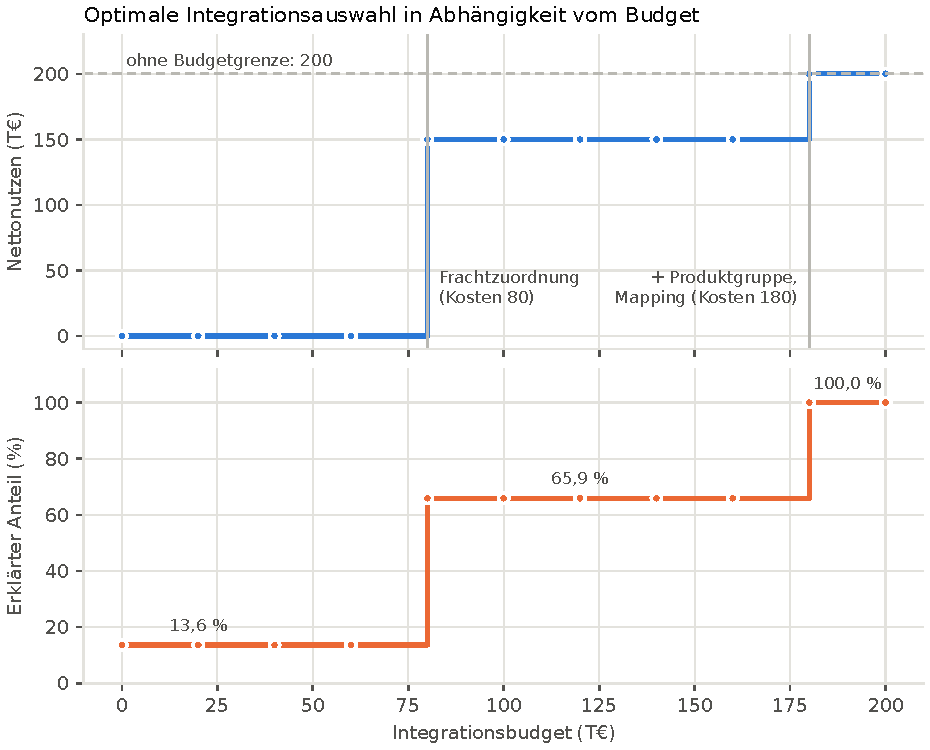
\includegraphics[width=0.85\linewidth]{abb_budget.pdf}
\caption{E2/E4: Nettonutzen der optimalen Auswahl (oben) und erklärter Anteil der Abweichung (unten) in Abhängigkeit vom Integrationsbudget. Kosten und Abhängigkeiten angenommen.}
\label{fig:e2}
\end{figure}

Abbildung~\ref{fig:e2} zeigt die Treppenform. In allen 12 Budgetstufen stimmt der Nettonutzen des Entscheiders mit der vollständigen Aufzählung überein. Rabatt-Feindaten werden nie ausgewählt. Die Laufzeit je Entscheidung lag zwischen 13{,}1 und 18{,}8\,ms (Median von je fünf Wiederholungen) und war damit praktisch unabhängig vom Budget.

\emph{Interpretation.} Die optimale Auswahl ist eine Treppenfunktion des Budgets mit zwei Schwellen. Die erste liegt bei 80\,T€, den Kosten der Frachtzuordnung; die zweite bei 180\,T€, den Summenkosten aus Fracht, Produktgruppe und Mapping. Aus der Messung folgt nur, dass die Schwellen in $(60,80]$ und $(160,180]$ liegen; ihre exakte Lage ergibt sich aus den angenommenen Kosten. Drei Beobachtungen sind inhaltlich relevant:
\begin{enumerate}
\item \textbf{Reihenfolge nach Nutzen-Kosten-Verhältnis.} Die Frachtzuordnung ($230$ Nutzen bei $80$ Kosten, Nettonutzen $+150$) hat Vorrang vor der Produktgruppe, die wegen des erforderlichen Mappings effektiv $100$ kostet und netto nur $+50$ bringt. Bei einem Budget von 100\,T€ ist die Frachtzuordnung allein (Netto 150) der Kombination aus Produktgruppe und Mapping (Netto 50) klar überlegen, obwohl der Einzelnutzen der Produktgruppe (150) und ihre isolierten Kosten (60) auf den ersten Blick ebenfalls für sie sprechen. Die Abhängigkeit verändert die Rangfolge. Eine Priorisierung, die nur Einzelposten betrachtet, würde hier falsch liegen.
\item \textbf{Schattenpreis des Budgets.} Ein Budget von 100 statt unbegrenzt kostet 50\,T€ Nettonutzen (150 statt 200). Zwischen 80 und 180\,T€ führt zusätzliches Budget zu keinem zusätzlichen Nutzen, danach springt der Nutzen um 50\,T€. Mehr Budget hilft nur, wenn es ein ganzes Paket erschließt.
\item \textbf{Nutzenlose Optionen werden nicht gewählt.} Die Rabatt-Feindaten haben im Modell den Nutzen 0 und werden deshalb nie ausgewählt. Das ist eine Folge der Annahme, nicht eine Aussage über ihren tatsächlichen Wert: Sie könnten für andere Fragen als die Margenabweichung nützlich sein, was das Modell mit einem einzigen Anwendungsfall nicht erfasst.
\end{enumerate}
Die Übereinstimmung mit der Aufzählung in allen 12 Fällen stützt die Korrektheit der Kodierung (Abhängigkeitsklauseln, Budgetvergleicher, Zielfunktion) für diese Instanz. Sie ist kein Korrektheitsbeweis; E3 erweitert die Prüfung.

\subsubsection{E3: Skalierung}
Tabelle~\ref{tab:e3} zeigt Laufzeit und Entscheideraufrufe für wachsende Instanzgrößen.

\begin{table}[htbp]
\centering
\small
\caption{E3: Laufzeit des SAT-basierten Entscheiders und der Aufzählung (Median über je 3 Instanzen; in Klammern Minimum bis Maximum des Entscheiders)}
\label{tab:e3}
\begin{tabular}{rrrrrr}
\toprule
$n$ & \textbf{Entscheider (ms)} & \textbf{Streuung (ms)} & \textbf{Aufzählung (ms)} & \textbf{Aufrufe} & \textbf{Faktor} \\
\midrule
4 & 30 & 28--30 & 0{,}04 & 16 & 795 \\
5 & 63 & 58--70 & 0{,}07 & 17 & 889 \\
6 & 129 & 61--137 & 0{,}15 & 18 & 836 \\
7 & 235 & 209--325 & 0{,}33 & 19 & 722 \\
8 & 519 & 330--710 & 0{,}57 & 21 & 910 \\
9 & 1\,320 & 460--1\,523 & 1{,}18 & 22 & 1\,115 \\
10 & 2\,616 & 1\,886--3\,154 & 2{,}70 & 23 & 969 \\
\bottomrule
\end{tabular}
\end{table}

\begin{figure}[htbp]
\centering
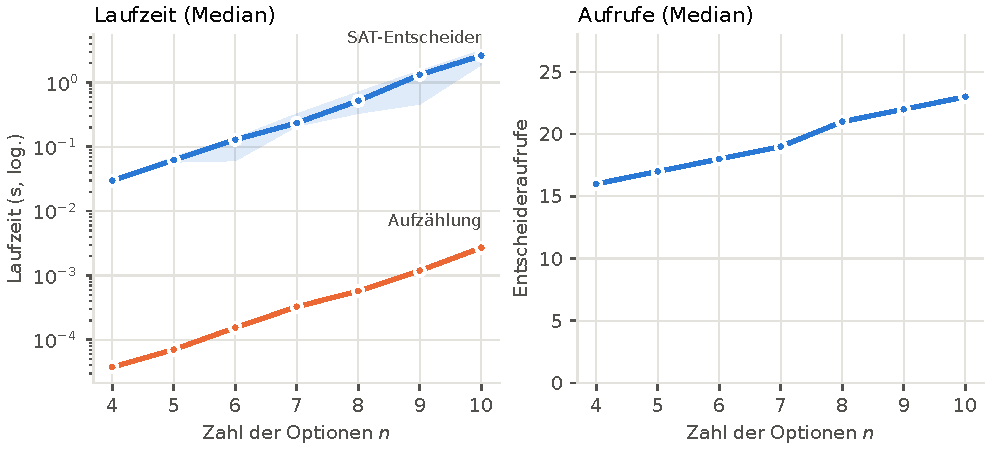
\includegraphics[width=0.95\linewidth]{abb_skalierung.pdf}
\caption{E3: Laufzeit (logarithmische Achse; Band: Minimum bis Maximum über 3 Instanzen) und Zahl der Entscheideraufrufe in Abhängigkeit von der Zahl der Optionen $n$.}
\label{fig:e3}
\end{figure}

\emph{Korrektheit.} In allen 21 Zufallsinstanzen stimmt der Nettonutzen des Entscheiders mit der Aufzählung überein.

\emph{Laufzeit.} Die Laufzeit des Entscheiders wächst exponentiell: Von $n=4$ auf $n=10$ steigt der Median von 30 auf 2\,616\,ms, also um den Faktor $\approx 87$, was einem Faktor von etwa $2{,}1$ je zusätzlicher Option entspricht (Einzelfaktoren zwischen $1{,}8$ und $2{,}5$). Die Zahl der Entscheideraufrufe wächst dagegen nur schwach (von 16 auf 23, etwa ein Aufruf mehr je Option); das ist mit einer Suche über den Wertebereich der Zielfunktion vereinbar, wurde hier aber nicht eigens untersucht. Der exponentielle Anteil liegt also nicht in der Zahl der Aufrufe, sondern im Aufwand je Aufruf. Die Streuung zwischen Instanzen gleicher Größe ist erheblich (bei $n=10$ von 1{,}9 bis 3{,}2\,s, also etwa $-28\,\%$ bis $+21\,\%$ um den Median). Da jede Instanz nur einmal gemessen wurde, lässt sich nicht trennen, wie viel davon auf die Struktur der Instanz und wie viel auf Messrauschen der geteilten Maschine entfällt.

\emph{Vergleich mit der Aufzählung.} Die einfache Aufzählung aller Teilmengen ist in diesem Größenbereich um etwa den Faktor 700 bis 1\,100 schneller als der Entscheider. Der Entscheider ist hier somit \emph{kein} Geschwindigkeitsgewinn. Dieser Befund ist ehrlich festzuhalten: Die Kodierung als Entscheider-Problem dient der formalen Anbindung an die Entscheiderbausteine des Referenzprojekts und der Prüfbarkeit, nicht der Rechenleistung. Auch die Aufzählung wächst mit $2^n$ und ist nur ein Referenzwert für kleine $n$. Für größere Portfolios sind spezialisierte Verfahren (zum Beispiel dynamische Programmierung für das Budgetproblem mit ganzzahligen Kosten oder ein ganzzahliger Optimierer) zu bevorzugen. Eine grobe Extrapolation (nicht gemessen) mit dem Faktor $2{,}1$ je Option ergäbe für $n=20$ eine Entscheiderlaufzeit in der Größenordnung von $2{,}6\,\mathrm{s}\cdot 2{,}1^{10}\approx 1\,\mathrm{h}$; die Extrapolation ist unsicher, weil nur sieben Größen und je drei Instanzen vorliegen.

\emph{Einordnung für die Praxis.} Ein Datennetz mit bis zu etwa zehn alternativen Integrationsvorhaben, wie es für ein einzelnes Data Product realistisch ist, lässt sich in Sekunden exakt optimieren. Entscheidend für die Qualität der Auswahl sind dann nicht die Rechenzeit, sondern die Schätzung von Nutzen und Kosten (siehe Abschnitt~\ref{sec:exp-grenzen}).

\subsubsection{E4: Erklärter Anteil bei schrittweiser Integration}
Wird angenommen, dass eine angebundene Quelle die zugehörige Ursache vollständig erklärbar macht, ergibt sich Tabelle~\ref{tab:e4}.

\begin{table}[htbp]
\centering
\small
\caption{E4: Erklärter Anteil der Abweichung von 440\,T€ nach schrittweiser Integration}
\label{tab:e4}
\begin{tabular}{p{0.40\linewidth}rrr}
\toprule
\textbf{Stufe} & \textbf{Erklärt (exakt)} & \textbf{Erklärt (\%)} & \textbf{Unerklärt (T€)} \\
\midrule
Ausgangslage (nur Rabatte) & $3/22$ & 13{,}64 & 380 \\
+ Frachtzuordnung & $29/44$ & 65{,}91 & 150 \\
+ Produktgruppe & $1$ & 100{,}00 & 0 \\
\bottomrule
\end{tabular}
\end{table}

\begin{figure}[htbp]
\centering
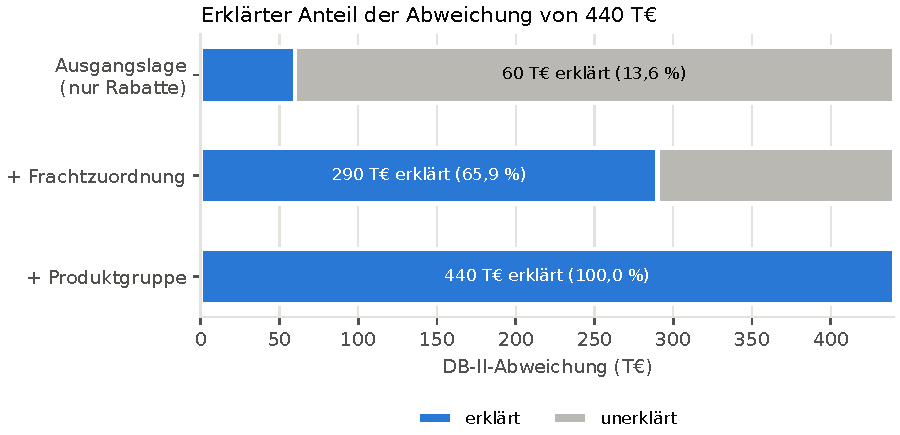
\includegraphics[width=0.85\linewidth]{abb_erklaerter_anteil.pdf}
\caption{E4: Erklärter und unerklärter Teil der DB-II-Abweichung von 440\,T€ nach schrittweiser Integration.}
\label{fig:e4}
\end{figure}

\emph{Interpretation.} Der erklärte Anteil steigt durch die Frachtzuordnung allein um etwa 52 Prozentpunkte; die zweite Integration schließt die verbleibenden 34 Prozentpunkte. Zusammen mit E2 lässt sich der Zusammenhang zwischen Budget und Aussagekraft ablesen: Unterhalb von 80\,T€ bleibt die Erklärung bei $13{,}6\,\%$, zwischen 80 und 180\,T€ bei $65{,}9\,\%$, ab 180\,T€ bei $100\,\%$. Für die Handlungsempfehlung der Fallstudie (Neuverhandlung mit einem Kunden mit 2{,}0\,Mio.\,€ Umsatz) wäre ein erklärter Anteil von $65{,}9\,\%$ wahrscheinlich noch zu gering, falls der Use-Case Owner ein strenges Error Budget festlegt; ein konkreter Schwellenwert wird hier bewusst nicht vorgegeben, da er fachlich zu bestimmen ist. Die Rechnung zeigt jedoch, dass die einfachste Integration (Fracht) den größten Fortschritt bringt, was mit der Rangfolge in E2 übereinstimmt.

Zu beachten ist, dass die 100\,\% eine \emph{obere Schranke} unter der Annahme vollständiger Erklärbarkeit nach Anbindung sind. Tatsächlich bleiben Definitionsabweichungen und zufällige Fehler (Fehlerzerlegung, Abschnitt~\ref{sec:formal}) bestehen, sodass der reale erklärte Anteil niedriger ausfallen kann.

\subsubsection{E5: Reproduzierbarkeit}
Fünf Wiederholungen von E1 lieferten identische Ergebnisprotokolle und denselben Fingerabdruck (SHA-256, Präfix \texttt{53eccfad}). Der Fingerabdruck bindet Name, Konfiguration, Eingaben und Versionen (einschließlich der Python-Version 3.13.16 und des Git-Standes des Referenzprojekts). Er ändert sich, sobald sich eine dieser Größen ändert.

\emph{Einschränkung.} Bitgleich reproduzierbar sind die rein rechnerischen Ergebnisse (E1, E4 und die Auswahlmengen in E2/E3). Die gemessenen Laufzeiten in E2 und E3 sind Teil der Ergebnisdateien, schwanken aber zwischen Läufen und sind nicht Teil des Fingerabdrucks. Wer die Laufzeiten vergleichen will, muss Hardware und Last berücksichtigen.

\subsection{Zusammenfassung der Befunde}
\begin{enumerate}
\item Die Implementierung reproduziert die Fallstudie exakt (E1). Der erklärte Anteil beträgt $3/22\approx 13{,}64\,\%$.
\item Der SAT-basierte Entscheider liefert in allen 33 geprüften Fällen (12 Budgetstufen und 21 Zufallsinstanzen) denselben Nettonutzen wie die vollständige Aufzählung (E2, E3).
\item Die optimale Integrationsauswahl ist eine Treppenfunktion des Budgets; Abhängigkeiten zwischen Quellen können die Rangfolge gegenüber einer Einzelbewertung umkehren (E2).
\item Die Laufzeit des Entscheiders wächst exponentiell, etwa um den Faktor $2{,}1$ je Option, und ist für kleine Instanzen etwa 700- bis 1\,100-mal langsamer als die naive Aufzählung (E3). Der Entscheider dient hier der formalen Anbindung, nicht der Geschwindigkeit.
\item Die Anbindung der Frachtdaten erhöht den erklärten Anteil von $13{,}6\,\%$ auf $65{,}9\,\%$ (E4).
\item Die rechnerischen Ergebnisse sind reproduzierbar, die Laufzeiten nicht bitgleich (E5).
\end{enumerate}

\subsection{Grenzen der Aussagekraft}
\label{sec:exp-grenzen}
Die Ergebnisse sind sorgfältig zu lesen:
\begin{itemize}
\item \textbf{Illustrative Daten.} Die Beträge der Fallstudie stammen aus einem Webinar und sind keine unabhängig erhobenen Unternehmensdaten. Die Integrationskosten und die Abhängigkeit vom Stammdaten-Mapping sind eigene Annahmen. Die Treppenschwellen (80 und 180\,T€) und die Nettonutzen (150, 200) sind damit \emph{Rechenbeispiele}, keine Empfehlungen für ein konkretes Unternehmen.
\item \textbf{Nutzen gleich Ursachenbetrag.} Der Nutzen einer Integration wurde mit dem vollen Betrag der dadurch sichtbaren Ursache gleichgesetzt. Das unterstellt, dass die Ursache nach der Anbindung vollständig vermieden oder korrigiert werden kann und dass die Posterior-Verteilung $\pi_1$ auf diesen Fall konzentriert ist. In der Praxis ist $\E_{\pi_1}[\Delta W]$ meist deutlich kleiner und selbst unsicher.
\item \textbf{Ein Anwendungsfall.} Das Modell bewertet Integrationen nur für eine einzelne Frage. Wiederverwendung über mehrere Anwendungen (Abschnitt~\ref{sec:data-product}) erhöht den Nutzen einer Integration und wird nicht abgebildet.
\item \textbf{Kleine Stichprobe.} E3 umfasst nur sieben Größen mit je drei Instanzen und eine einzige Messung je Instanz. Konfidenzintervalle wurden nicht berechnet; die Faktoraussagen sind Größenordnungen.
\item \textbf{Messumgebung.} Die Messungen stammen aus einer geteilten virtuellen Maschine mit zwei Kernen; absolute Zeiten sind auf anderer Hardware nicht übertragbar, das exponentielle Muster dagegen schon.
\item \textbf{Testabdeckung.} Die 72 Tests bestätigen die Funktionalität, aber die Abdeckungsmessung wurde nicht ausgeführt; die Aussage „alle Tests bestehen“ ist daher keine Aussage über den Grad der Abdeckung.
\end{itemize}

\subsection{Reproduktion}
Die Experimente liegen als Skript \texttt{src/experiments.py} im Projekt; Ergebnisse stehen als JSON-Dateien im Verzeichnis \texttt{src/results/}, die Abbildungen (erzeugt mit \texttt{src/plots.py}) in \texttt{src/results/plots/} und als Kopie in \texttt{science/}. Nach Installation (\texttt{pip install -e ".[dev]"}) wird das Skript aus dem Projektwurzelverzeichnis mit
\begin{quote}
\texttt{python src/experiments.py}
\end{quote}
und anschließend mit \texttt{python src/plots.py} die Abbildungen erzeugt.
ausgeführt. Die Gesamtlaufzeit beträgt auf der in Tabelle~\ref{tab:hardware} beschriebenen Umgebung etwa 15\,s.

\section{Diskussion, Grenzen und Ausblick}
\label{sec:discussion}

\subsection{Einordnung der Befunde}
Die Arbeit verbindet drei Ebenen: ein begriffliches Modell (Datennetz, Data Product, Provenance, Stakes), eine ökonomische Bedingung (Error Budget, VOI) und eine ausführbare Umsetzung, die an der Fallstudie und an synthetischen Instanzen geprüft wurde (Abschnitt~\ref{sec:experiment}). Die Ebenen stützen sich gegenseitig, aber nicht gleich stark. Die Fallstudie ist illustrativ, die Experimente zeigen die \emph{interne Konsistenz} und das \emph{Rechenverhalten} des Modells, nicht seine \emph{empirische Wirksamkeit} in einem realen Unternehmen. Ein bestandener Test und eine reproduzierte Zahl belegen, dass die Formeln richtig umgesetzt sind; sie belegen nicht, dass die Annahmen hinter den Formeln in der Praxis gelten.

Drei Ergebnisse der Experimente verdienen eine ausdrückliche Einordnung.
\begin{enumerate}
\item \textbf{Abhängigkeiten dominieren die Rangfolge.} Im Rechenbeispiel (E2) ist die Frachtzuordnung die beste erste Investition, obwohl der Einzelnutzen der Produktgruppe auf den ersten Blick ähnlich attraktiv wirkt. Der Grund liegt im verdeckten Voraussetzungsaufwand: Wer nur Einzelposten betrachtet, überschätzt Vorhaben mit versteckten Abhängigkeiten. Für die Praxis folgt daraus kein konkreter Zahlenwert, wohl aber eine Methodenregel: Integrationsvorhaben sind mit ihren Vorleistungen zu bewerten, nicht isoliert.
\item \textbf{Der Nutzen ist treppenförmig, nicht stetig.} Zusätzliches Budget führt nur dann zu zusätzlichem Nutzen, wenn es ein ganzes Paket erschließt (E2). Das legt nahe, Budgetentscheidungen an \emph{Schwellen} zu orientieren, statt Mittel gleichmäßig zu verteilen; ob reale Datenprojekte eine solche Schwellenstruktur zeigen, ist empirisch zu prüfen.
\item \textbf{Der Rechenaufwand liegt nicht dort, wo man ihn zuerst vermutet.} Der SAT-basierte Entscheider benötigt nur wenige Aufrufe, aber jeder Aufruf wird mit wachsender Optionszahl etwa doppelt so teuer (E3). Für die kleinen Portfolios eines einzelnen Data Products ist das unkritisch; der Entscheider ist jedoch ein Mittel zur formalen Anbindung an das Referenzprojekt und kein Geschwindigkeitsvorteil gegenüber einer einfachen Aufzählung.
\end{enumerate}
Der erklärte Anteil der Fallstudie (E4) zeigt zudem, dass die größte Verbesserung mit der \emph{ersten} Integration entsteht: Die Anbindung der Frachtdaten allein hebt den erklärten Anteil von $13{,}6\,\%$ auf $65{,}9\,\%$. Das ist plausibel, weil der Frachtanteil der größte Posten ist; es ist jedoch ein Befund des konkreten Zahlenbeispiels und keine allgemeine Gesetzmäßigkeit abnehmender Grenzerträge.

\subsection{Grenzen des Modells}
Die formalen Modelle vereinfachen reale Unternehmens\-prozesse bewusst: Einfluss\-beziehungen sind nicht immer linear, Referenzwerte können selbst unsicher sein und Ursachen interagieren. Auch die im Fallbeispiel genannten Beträge sind eine illustrative Webinar-Fallstudie und keine unabhängig erhobene Unternehmensanalyse. Die angegebenen Reife- und Fehlermaße müssen daher als fallbezogene Entscheidungshilfen verstanden werden.

Eine weitere Grenze ist die Auswahl der Testfragen. Ein hoher Messwert für leicht beantwortbare oder häufige Fragen sagt wenig über seltene, aber folgenreiche Ausnahmen aus. Testsets sollten deshalb nach möglichen Auswirkungen geschichtet und auch nach Änderungen an Datenquellen, Definitionen, Modellen oder Berechtigungen erneut ausgeführt werden. Ebenso ist eine Abweichung nicht automatisch ein Beleg gegen das Datennetz: Sie kann auf einen Fehler in der internen Analyse, eine andere zulässige Definition oder einen inzwischen veränderten Datenstand hinweisen.

Aus den Experimenten kommen folgende Grenzen hinzu:
\begin{itemize}
\item \textbf{Annahmen statt Messungen.} Integrationskosten, die Abhängigkeit vom Stammdaten-Mapping und die Gleichsetzung von Nutzen und Ursachenbetrag sind Annahmen. Die Treppenschwellen von 80 und 180\,T€ und die Nettonutzen von 150 und 200\,T€ sind Rechenbeispiele und keine Prognose für ein Unternehmen.
\item \textbf{Deterministische Nutzen.} Das Experiment behandelt den erwarteten Nutzen $\E_{\pi_1}[\Delta W]$ als bekannte Zahl. Tatsächlich ist dieser Wert selbst unsicher; ein Entscheider sollte Unsicherheitsbereiche und nicht nur Punktwerte verarbeiten.
\item \textbf{Vollständige Erklärbarkeit als Obergrenze.} Der erklärte Anteil von $100\,\%$ nach beiden Integrationen setzt voraus, dass jede angebundene Quelle ihre Ursache vollständig erklärbar macht. Definitionsabweichungen und zufällige Fehler (Abschnitt~\ref{sec:error}) bleiben bestehen.
\item \textbf{Ein Anwendungsfall.} Die Wiederverwendung eines Data Products über mehrere Anwendungen (Abschnitt~\ref{sec:data-product}) erhöht den Nutzen einer Integration, wird im Experiment aber nicht abgebildet; der Einzelfallnutzen unterschätzt daher tendenziell den Gesamtnutzen.
\item \textbf{Kleine Stichproben und eine Messumgebung.} Die Skalierungsmessung umfasst sieben Instanzgrößen mit je drei Instanzen, jede einmal gemessen, auf einer einzelnen geteilten virtuellen Maschine. Die Aussage „etwa Verdopplung je Option“ ist eine Größenordnung, die absoluten Zeiten gelten nur für diese Umgebung.
\item \textbf{Keine Messung mit realen KI-Antworten.} Die Experimente rechnen mit dem Modell; sie bewerten keine tatsächlichen Antworten eines KI-Systems gegen Referenzfälle. Die Kennzahlen der Testfragen (Bestehensquote, Provenance-Abdeckung) wurden somit nur durch Einheitstests, nicht an realen Daten geprüft.
\end{itemize}

Die wirtschaftliche Logik bleibt dennoch belastbar: Datenverbesserungen sollten dort priorisiert werden, wo ihr erwarteter zusätzlicher Nutzen die Integrations- und Betriebskosten rechtfertigt. In der Praxis sind dafür kontrollierte Experimente, historische Was-wäre-wenn-Analysen und eine nachvollziehbare Messung der Folgen nötig. Die Schätzung dieses Nutzens in realen Geschäftsfällen bleibt eine zentrale offene Aufgabe.

\subsection{Ausblick}
Aus den Grenzen ergeben sich konkrete Arbeitsfelder, die sich in vier Gruppen ordnen lassen: Erhebung realer Daten, Erweiterung des Modells, bessere Rechenverfahren und Betrieb in der Praxis.

\subsubsection{Empirische Validierung mit realen Daten}
\begin{enumerate}
\item \textbf{Mehrere reale Fallstudien.} Die Arbeit stützt sich auf einen illustrativen Einzelfall. Sinnvoll sind Fallstudien in mehreren Unternehmen und Branchen, in denen die DB-II-Abweichung (oder eine andere Kennzahl) tatsächlich von Controlling-Fachleuten zerlegt und mit der Antwort eines KI-Systems verglichen wird. Daraus ließen sich die Verteilung des erklärten Anteils und die typischen Ursachenklassen empirisch bestimmen, statt sie an einem Beispiel zu illustrieren.
\item \textbf{Vorher-Nachher-Messung.} Der Kern der These ist, dass Integrationen den erklärten Anteil und damit die Verlässlichkeit erhöhen. Das ließe sich testen, indem der erklärte Anteil vor und nach einer konkreten Integration (zum Beispiel der Verknüpfung von Fracht und Auftrag) mit denselben Testfragen gemessen wird. Aussagekräftig wäre ein Vergleich mit einer Kontrollgruppe von Fragen oder Bereichen ohne Integration.
\item \textbf{Auswertung realer KI-Antworten.} Die Kennzahlen der Testfragen (gewichtete Bestehensquote, Provenance-Abdeckung, Anteil unbeantworteter Fragen) sollten an Antworten verschiedener Systeme und Modellversionen erhoben werden. Von Interesse ist insbesondere, ob sich der Befund der Fallstudie bestätigt, dass bei gleichem Datennetz ein Modellwechsel die Lücken nicht schließt.
\item \textbf{Schätzung von Nutzen und Kosten.} Statt angenommener Werte sind historische Was-wäre-wenn-Analysen nötig: Was hätte eine früher vorhandene Frachtverknüpfung gekostet, und welche Fehlentscheidung hätte sie vermieden? Erst damit wird die VOI-Bedingung $\E_{\pi_1}[\Delta W]\ge C_{int}$ zahlenmäßig belastbar.
\end{enumerate}

\subsubsection{Erweiterungen des Modells}
\begin{enumerate}
\item \textbf{Unsicherheit im Nutzen.} Der Nutzen einer Integration lässt sich als Zufallsvariable modellieren. Die Auswahl könnte dann den Erwartungswert, einen Quantilswert oder eine Risikoaversion berücksichtigen; eine Sensitivitätsanalyse über Kosten und Nutzen würde zeigen, wie robust die Treppenschwellen sind und welche Annahme das Ergebnis am stärksten bestimmt.
\item \textbf{Teilweise Erklärbarkeit.} Der Baustein für Ursachen erlaubt bereits erklärte Anteile zwischen 0 und 1. Das Experiment nutzt nur die Extremwerte. Eine Erweiterung könnte den Erklärungsgrad einer Quelle von ihrer Qualität, Aktualität und Granularität abhängig machen und damit die Verbindung zur Fehlerzerlegung (fehlende Treiber, Definitionsabweichung, Zufallsfehler) herstellen.
\item \textbf{Mehrere Anwendungsfälle und gemeinsame Quellen.} Ein Data Product bedient mehrere Anwendungen. Das Modell sollte den Nutzen einer Integration über alle Anwendungen summieren und gemeinsame Vorleistungen nur einmal bepreisen; das würde die im Text behauptete Wiederverwendungswirkung quantifizierbar machen.
\item \textbf{Zeitliche Abfolge und Lernen.} Integrationen erfolgen nacheinander, und jede Abweichung verändert den Posterior über den Zustand des Datennetzes (Abschnitt~\ref{sec:opportunity}). Ein dynamisches Modell würde die Reihenfolge der Integrationen und den Wert des Wartens bewerten und den Lern-Loop mit dem Bayes-Update ausdrücklich in die Auswahl einbeziehen.
\item \textbf{Verbindung zur Governance.} Die Vertrauensstufen und Freigabehindernisse sind bisher getrennt vom Integrationsproblem. Man könnte untersuchen, welche Integrationen nötig sind, um eine Anwendung von Stufe~1 auf Stufe~3 zu heben, und wie sich dabei Error Budget, Stakes und Kosten verhalten.
\end{enumerate}

\subsubsection{Rechenverfahren}
Das Auswahlproblem mit Budget enthält ohne Abhängigkeiten das Rucksackproblem und ist deshalb im Allgemeinen NP-schwer; die Experimente zeigen das exponentielle Verhalten des gewählten Entscheiders. Für größere Portfolios sind spezialisierte Verfahren naheliegend: dynamische Programmierung über ganzzahlige Kosten, ganzzahlige lineare Optimierung oder Heuristiken mit Gütegarantie. Der SAT-basierte Entscheider könnte dabei als \emph{Referenz zur Prüfung} der schnelleren Verfahren dienen, wie es die Aufzählung hier für den Entscheider tut. Eine systematische Messung mit mehr Instanzen, Wiederholungen je Instanz, Konfidenzintervallen und auf mehreren Hardware-Konfigurationen würde die Laufzeitaussagen von Größenordnungen auf belastbare Schätzungen heben.

\subsubsection{Betrieb und Nachvollziehbarkeit}
\begin{enumerate}
\item \textbf{Kontinuierliche Prüfung.} Testfragen und Kennzahlen sollten als wiederkehrender Lauf im Betrieb ausgeführt werden, damit Änderungen an Quellen, Definitionen oder Modellen automatisch auffallen. Das Experimentprotokoll mit Fingerabdruck ist dafür ein Baustein; es müsste um Versionierung der Testdaten und der Referenzwerte ergänzt werden.
\item \textbf{Reproduzierbare Umgebung.} Die Experimente wurden mit einem per Git eingebundenen Referenzprojekt und ohne Abdeckungsmessung ausgeführt. Eine festgelegte Umgebung (Container oder gesperrte Abhängigkeiten) und eine automatische Ausführung der Tests mit Abdeckungsbericht würden die Nachprüfbarkeit verbessern.
\item \textbf{Organisatorische Verankerung.} Die drei Verantwortlichkeiten (Data Owner, Data Product Owner, Use-Case Owner) wurden begrifflich eingeführt. Offen ist, wie sie in verschiedenen Organisationsformen tatsächlich besetzt werden und wie sich die Entscheidungen über Integrationen und Freigaben dokumentieren und auditieren lassen.
\item \textbf{Regulatorischer Rahmen.} Die vier Vertrauensstufen sind ein konzeptioneller Rahmen und keine Norm. Ihre Beziehung zu branchenspezifischen Anforderungen (etwa an Nachvollziehbarkeit, menschliche Aufsicht und Dokumentation) wäre getrennt zu untersuchen.
\end{enumerate}

\subsubsection{Offene Forschungsfragen}
Aus alledem ergeben sich fünf Fragen, die diese Arbeit nicht beantwortet, aber präzise formuliert:
\begin{enumerate}
\item Wie verteilt sich der erklärte Anteil einer KI-Antwort in realen Unternehmen vor und nach gezielten Integrationen?
\item Wie robust ist die ökonomisch optimale Integrationsreihenfolge gegenüber Unsicherheit in Kosten und Nutzen?
\item Wie lässt sich der Nutzen eines wiederverwendbaren Data Products über mehrere Anwendungen belastbar zurechnen?
\item Welche Anforderungen an Nachweis und Aufsicht rechtfertigen den Übergang zwischen den Vertrauensstufen, und wie lassen sie sich messen?
\item Welche Rechenverfahren sind für Portfolios mit Dutzenden Integrationsvorhaben geeignet, und wie lassen sie sich gegen eine exakte Referenz prüfen?
\end{enumerate}

\section{Schlussfolgerung}
\label{sec:conclusion}

\subsection{Beantwortung der Leitfrage}
Die Frage „Wann ist das Datennetz gut genug für KI?“ hat keine allgemeingültige, absolute Schwelle. Gut genug ist es für einen bestimmten Anwendungsfall, wenn relevante Einflussgrößen verknüpft und definiert sind, Qualität und Aktualität bekannt sind, Antworten nachvollziehbare Provenance tragen und der verbleibende Fehler im Verhältnis zu den Stakes vertretbar ist. Die Arbeit liefert dafür keine Zahl, sondern ein \emph{Verfahren}: die Frage und ihre Folgen bestimmen das Error Budget, das Datennetz bestimmt, wie viel der Abweichung erklärt werden kann, und die Differenz wird dort geschlossen, wo der erwartete Nutzen die Kosten übersteigt.

\subsection{Zusammenfassung der Arbeit}
\paragraph{Ausgangspunkt und These.}
Viele Unternehmen setzen KI früher ein, als ihre Daten dafür reif sind. Die Arbeit argumentiert, dass die Verlässlichkeit einer KI-Antwort nicht nur vom Modell, sondern ebenso von Zugänglichkeit, Verknüpfung, Definition und Aktualität der Daten abhängt, und dass Perfektion weder erreichbar noch nötig ist. Entscheidend ist, ob der verbleibende Fehler für den Verwendungszweck klein genug ist. Abweichungen zwischen KI-Antwort und interner Analyse sind dabei nicht nur ein Risiko, sondern ein Diagnosesignal, das Datenlücken und zugleich Lücken in der eigenen Analyse sichtbar machen kann.

\paragraph{Fallstudie.}
Die illustrative Fallstudie eines Maschinenbauzulieferers zeigt eine DB-II-Abweichung von 440\,T€. Die KI erklärte durch den Rabattanstieg nur 60\,T€, also $3/22\approx 13{,}6\,\%$; die beiden größeren Ursachen, Expressfracht (230\,T€) und Produktmix (150\,T€), waren im zugänglichen Datennetz nicht verknüpft oder nicht vorhanden. Eine auf die plausible, aber unvollständige Antwort gestützte Maßnahme hätte einen wichtigen Kunden belastet, ohne die Hauptursache zu treffen. Die Lücke lag im Datennetz, nicht im Sprachmodell.

\paragraph{Formales Modell.}
Das Datennetz wird als gerichteter Multigraph modelliert, ein Data Product als wiederverwendbarer Teil mit Daten, Bedeutung und Label. Die Fehlerzerlegung unterscheidet fehlende Einflussgrößen, Definitionsabweichungen und zufällige Fehler. Die Gut-genug-Bedingung bindet den erwarteten Verlust an die Stakes und ein anwendungsbezogenes Error Budget: $\E[L(\hat y,y^*)]\le\varepsilon W$. Die Abweichung zwischen KI-Antwort und interner Analyse wird als Bayesscher Indikator über den Zustand des Datennetzes gedeutet; die VOI-Bedingung $\E_{\pi_1}[\Delta W]\ge C_{int}$ entscheidet, ob sich eine Integration lohnt.

\paragraph{Vertrauensstufen und Verantwortung.}
Vier Stufen (Hinweis, Gegenprüfung, Entscheidungsvorbereitung, automatisierte Handlung) ordnen den Einsatz von KI nach den Folgen eines Fehlers; eine höhere Stufe setzt belegbaren Reifegrad voraus und ergibt sich nicht automatisch aus bisherigem Erfolg. Bedeutung, Lieferung und Freigabe sind drei getrennte Verantwortlichkeiten mit benannten Personen (Data Owner, Data Product Owner, Use-Case Owner).

\paragraph{Praktisches Vorgehen.}
Das schrittweise Vorgehen beginnt mit einer konkreten Frage und deren Stakes, baut ein Data Product in kleinen Schritten auf, misst Fortschritt mit getrennten Kennzahlen (Bestehensquote, Provenance-Abdeckung, erklärter Anteil, Vollständigkeit kritischer Attribute, Aktualität) und endet in einer Go-live-Checkliste. Mittelstand und Großunternehmen setzen unterschiedliche Schwerpunkte.

\paragraph{Experimentelle Befunde.}
Die Umsetzung als ausführbares Modell (72 Tests, alle bestanden) wurde an fünf Experimenten geprüft (Abschnitt~\ref{sec:experiment}):
\begin{enumerate}
\item Die Fallstudie wird exakt reproduziert; der erklärte Anteil beträgt $3/22\approx 13{,}64\,\%$.
\item Der Entscheider stimmt in allen 33 geprüften Fällen (12 Budgetstufen, 21 Zufallsinstanzen) mit einer vollständigen Aufzählung im Nettonutzen überein.
\item Die optimale Integrationsauswahl ist eine Treppenfunktion des Budgets: bis 60\,T€ keine Integration, ab 80\,T€ die Frachtzuordnung (Nettonutzen 150\,T€), ab 180\,T€ zusätzlich Produktgruppe und Mapping (Nettonutzen 200\,T€). Abhängigkeiten zwischen Quellen können die Rangfolge gegenüber einer Einzelbewertung umkehren.
\item Die Anbindung der Frachtdaten hebt den erklärten Anteil von $13{,}6\,\%$ auf $65{,}9\,\%$; die Produktgruppe schließt die Lücke unter der Annahme vollständiger Erklärbarkeit.
\item Der SAT-basierte Entscheider verdoppelt seine Laufzeit etwa je zusätzlicher Option (30\,ms bei $n=4$, 2{,}6\,s bei $n=10$) und ist für kleine Instanzen 700- bis 1\,100-mal langsamer als die naive Aufzählung; er dient der formalen Anbindung, nicht der Geschwindigkeit.
\item Die rechnerischen Ergebnisse sind reproduzierbar (gleicher Fingerabdruck in fünf Läufen); gemessene Zeiten sind es nicht bitgleich.
\end{enumerate}
Alle Messungen stammen aus einer geteilten virtuellen Maschine mit zwei Kernen und 7{,}8\,GiB Arbeitsspeicher (Tabelle~\ref{tab:hardware}); die Kosten- und Abhängigkeitsannahmen sind Rechenbeispiele.

\subsection{Praktische Folgerungen}
Aus Fallstudie, Modell und Experimenten folgen sechs Kernaussagen:
\begin{enumerate}
\item Die Qualität einer KI-Erklärung hängt maßgeblich von den verfügbaren Daten, ihren Verbindungen und ihrer fachlichen Bedeutung ab, nicht allein vom Modell.
\item „Gut genug“ ist eine wirtschaftliche und anwendungsbezogene Bedingung: Je folgenreicher die Entscheidung, desto stärker müssen Fehler begrenzt und belegt werden.
\item Vertrauen lässt sich schrittweise aufbauen – durch klare Definitionen, messbare Qualität, Provenance und benannte Verantwortliche.
\item KI kann bereits heute als Hinweis und Gegenprüfung nützlich sein. Eine Abweichung zeigt mögliche Datenlücken auf, kann aber ebenso eine unvollständige eigene Analyse offenlegen.
\item Ein Data Product schafft eine wiederverwendbare Grundlage für verschiedene Anwendungen; der Aufwand für gemeinsame Daten und Definitionen kann dadurch mehrfach Nutzen stiften.
\item Vor einem Go-live müssen fachliche Definition, technische Lieferung und Freigabe des konkreten Anwendungsfalls jeweils einer verantwortlichen Person zugeordnet sein.
\end{enumerate}
Die Experimente ergänzen drei Hinweise für die Priorisierung von Datenprojekten: Integrationen sind mit ihren Vorleistungen zu bewerten; Budgetentscheidungen sollten Schwellen beachten, an denen ein ganzes Paket erschlossen wird; und die erste Integration mit dem größten Ursachenanteil bringt meist den größten Fortschritt, was im Einzelfall zu prüfen ist.

Für die beteiligten Rollen bedeutet das Folgendes:
\begin{description}[style=nextline]
\item[Controlling und Fachbereich.] Abweichungen zwischen KI-Antwort und eigener Analyse systematisch als Diagnoseanlass nutzen, den erklärten Anteil als Kennzahl führen und Empfehlungen mit hohen Folgen nicht auf einen niedrigen erklärten Anteil stützen.
\item[Data Product Owner.] Integrationsvorhaben mit Kosten, Nutzen und Abhängigkeiten bewerten und nach Nutzen-Kosten-Verhältnis unter Einschluss der Vorleistungen ordnen; Vollständigkeit kritischer Attribute und Aktualität überwachen.
\item[Use-Case Owner.] Error Budget und Testfragen festlegen, nach Stakes schichten, und die Freigabe einer höheren Vertrauensstufe an Nachweise knüpfen.
\item[Management.] Die Frage nach dem Modell durch die Frage nach der Datenlage für die konkrete Entscheidung ergänzen und Datenarbeit als Investition mit erwartetem Nutzen statt als Nebenaufgabe behandeln.
\end{description}

\subsection{Schlussbemerkung}
Die Arbeit ist ein konzeptioneller und methodischer Beitrag mit einer geprüften Umsetzung, kein empirischer Wirksamkeitsnachweis. Ihr Wert liegt darin, die Frage nach der Eignung des Datennetzes präzise zu stellen, ökonomisch zu begründen und rechnerisch nachprüfbar zu machen. Die Belastbarkeit der Zahlen hängt von der Qualität der Annahmen ab; der Ausblick benennt, wie sie durch reale Daten ersetzt werden können.

\begin{quote}
\textbf{Leitgedanke:} Nicht nur fragen, ob die KI gut genug ist, sondern ob das Datennetz für diese Frage gut genug ist. Bis dahin die KI als Hinweis nutzen, ihre Antworten mit der eigenen Analyse abgleichen und aus jeder Abweichung lernen.
\end{quote}

\section*{Danksagung}
Die Arbeit basiert auf den Ideen und Folien von ai-data-network-economic-approach-en.md sowie auf den wissenschaftlichen Vorarbeiten des Autors zur wirtschaftlichen Bewertung eines SAT-Solvers und zu Wirtschaftssystemen unter Unsicherheit \cite{sat2026,uncertainty2026}.

\appendix
\section{Glossar}
\begin{description}[style=nextline]
\item[Datennetz] Gesamtheit der Unternehmensdaten und der fachlichen sowie technischen Verbindungen zwischen ihnen.
\item[Data Product] Wiederverwendbare Einheit aus Daten, ihrer Bedeutung und einem Label mit Nutzungsvoraussetzungen und benannter Verantwortung.
\item[DB\,I / DB\,II] Deckungsbeitrag I beziehungsweise II. In der Fallstudie bezeichnet „Marge“ die DB-II-Marge.
\item[Data Owner] Fachlich verantwortliche Person für Bedeutung und Definition von Kennzahlen.
\item[Data Steward] Unterstützt den Data Owner bei der laufenden Pflege und Anwendung fachlicher Regeln.
\item[Data Product Owner] Verantwortet die Lieferung, Vollständigkeit, Aktualität, Prüfung und Berechtigung des Data Products.
\item[Use-Case Owner] Verantwortet Freigabe und Testfragen einer KI-Anwendung, ihr Error Budget und die Grenze menschlicher Entscheidungen.
\item[Granularität] Detailstufe eines Datensatzes, beispielsweise eine Zeile je Auftragsposition.
\item[Provenance] Nachvollziehbare Angaben zu Definition, Quelle, Version und Datenstichtag einer Antwort.
\item[Error Budget] Für einen Anwendungsfall zulässiger Fehler, bestimmt durch Stakes und mögliche Folgen.
\item[Gegenprüfung (Cross-check)] Vergleich einer KI-Antwort mit eigener Analyse, Strategie oder fachlich geprüfter Referenz.
\item[MCP] Model Context Protocol; ein Standard, über den KI-Anwendungen auf Daten und Werkzeuge zugreifen können.
\item[Integrationsoption] Mögliche Anbindung einer Datenquelle oder eines Attributs mit erwartetem Nutzen, Kosten und gegebenenfalls benötigten Vorleistungen (Abschnitt~\ref{sec:experiment}).
\item[Nettonutzen] Differenz aus erwartetem Nutzen und Integrationskosten einer Auswahl von Integrationsoptionen.
\item[Erklärter Anteil] Anteil einer bekannten Abweichung, den eine Antwort durch sichtbare Ursachen erklärt.
\item[Value of Information (VOI)] Erwarteter zusätzlicher Nutzen einer Information oder Datenverbesserung im Vergleich zu ihren Kosten.
\end{description}

\section{Formale Beweise und Erweiterungen}
\subsection{Erweiterung: Nichtlineare Einflussmodelle}
Die lineare Darstellung kann durch eine allgemeine nichtlineare Regressionsdarstellung $y^*=g(S_q)$ mit Lipschitz-Bedingung $(\exists L: |g(x)-g(x')|\le L\|x-x'\|)$ verallgemeinert werden. Dann gilt eine analoge Fehlerabschätzung:
\[
|\hat y-y^*| \le L\cdot \|S_q-\tilde S_q\| + |B_{def}| + |\eta|.
\]

\subsection{Beweisskizze: VOI-Berechnung}
Mit Posterior $\pi_1(\theta)$ ist der erwartete Wert der Integration eines zusätzlichen Datenobjekts $z$:
\[
\E_{\pi_1}[\Delta W] = \sum_{\theta} \pi_1(\theta) \big( W(\text{with }z,\theta)-W(\text{without }z,\theta)\big).
\]
Dies kann numerisch über Simulation oder historische "what-if"-Analysen geschätzt werden.

\bibliographystyle{plain}
\begin{thebibliography}{9}
\bibitem{webinar2026} Michael Sullmann (BE-terna), Webinar "Data Product and AI in Controlling", Okt 2026.
\bibitem{sat2026} Stephan Epp. \emph{Wirtschaftliche Konsequenzen eines effizienten SAT-Solvers}. 12. Oktober 2026. \url{https://github.com/naphz86/subgraph-sat-solver-econ}.
\bibitem{uncertainty2026} Stephan Epp. \emph{Wirtschaftssysteme unter Unsicherheit}. 3. September 2026. \url{https://github.com/naphets86/odd/tree/main/science/uncrtecos}.
\end{thebibliography}

\end{document}
